\chapter{Quasar Emission Lines as Probes of Orientation and Unification}

%% Codes
\def\py{\textsc{python}}
\def\tar{\textsc{tardis}}
\def\cld{\textsc{cloudy}}
\def\agn{\textsc{agnspec}}
\def\kerrtrans{\textsc{kerrtrans}}


%% Lines and ions
\def\civ{C~\textsc{iv}}
\def\nv{N~\textsc{v}}
\def\heii{He~\textsc{ii}}
\def\ovi{O~\textsc{vi}}
\def\la{Ly$\alpha$}
\def\ha{H$\alpha$}
\def\oiii{O~\textsc{iii}}
\def\oiiifull{O~\textsc{iii}~5007\AA}
\def\fwh{FWHM[H$\beta$]}
\def\ewo{EW[O~\textsc{iii}]}
\def\ept{$\epsilon(\theta)$}

%% Journal definitions
\def\araa{ARAA}
\def\nat{Nature}
\def\apjl{ApJ Letters}
\def\aapr{AAPR}
\def\ssr{SSR}
\def\apj{ApJ}
\def\apjs{ApJs}
\def\pasp{PASP}
\def\aap{A\&A}
\def\mnras{MNRAS}
\def\aj{AJ}
\def\rmxaa{RMXAA}
\def\ew{{\rm EW}}

{\em This chapter is based on a paper in prepation:

Matthews J. H., Knigge C., 
`Quasar Emission Lines as Probes of Orientation and Unification',
to be submitted to MNRAS.}


%%%%%%%%%%%%%%%%%%%%%%%%%%%%%%%%%%%%%%
%
%          ABSTRACT
%
%%%%%%%%%%%%%%%%%%%%%%%%%%%%%%%%%%%%%%%
\maketitle

\section{Introduction}

In the previous chapter, I presented tests of geometric unification
models using MCRT and photoionization simulations. 
One of the key results from that analysis is that trends with
inclination prohibit models with equatorial outflows matching
observations, as the EW of the emission lines tend
to increase with inclination. This trend has clear implications for
the geometries of BAL outflows; the viewing angle may determine many
of the selection effects at work and must therefore be understood
before the true covering factor of BAL outflows can be accurately 
determined. The covering factor and opening angle of the outflow
are important quantities to measure in order to calculate the
feedback efficiency \citep[e.g.][]{borguet2012}, 
and make inferences about the outflow physics \citep[e.g.][]{proga2005}. 

Unlike in galactic accretion disc systems, measuring inclinations
for quasars and AGN is notoriously difficult, and obtaining 
reliable orientation indicators is thus an important observational
goal for the community. Perhaps as a result of this problem, 
directly opposing geometries have been proposed for 
BAL outflows (see section~??). Here, I use observational 
data from the Sloan Digital Sky Survey to constrain the inclinations
of BAL quasars. Similar attempts have been made previously with
different diagnostics; for example, by considering 
radio properties \citep{zhou2006,dipompeo2012a}, 
polarisation \citep{brotherton2006}
and general emission line properties \citep{dipompeo2012b}.  

This chapter is structured as follows. First, I describe
the data sample and selection criteria being used. I begin by
simply examining the distributions of the EW of the \oiiifull\ emission line,
\ewo, and comparing the BAL and non-BAL quasar distributions. 
In section~\ref{sec:disc_agn} I review the angular distribution of 
continuum emission one would expect from simple $\alpha$-disc models, 
as well as exploring the same quantity in more advanced disc models computed
with \agn. I then use these theoretical 
angular distributions applied to a simple toy model in 
section~\ref{sec:mc_angular},
and conduct MC simulations in an attempt to fit the observed BAL and non-BAL
quasar distributions of \ewo, using a similar approach to 
\citet[][hereafter R11]{risaliti2011}. 
In section~\ref{sec:discuss_ew} I discuss the results
in the context of radio and polarisation measurements of AGN, as well
as exploring the location of BAL quasars in `Eigenvector 1' parameter space.
Finally, in section~\ref{sec:ew_conclusions}, I summarise the findings.

% {\bf{\sl{\huge Abstract}}}

% The incidence of broad absorption lines (BALs) in quasar samples is 
% often explained by a geometric unification model consisting
% of an accretion disc and an associated outflow.
% This outflows is assumed to have a covering factor roughly equivalent to
% the BAL fraction, $f_{BAL}$. We test this model
% by examining ultraviolet (UV) emission line equivalent-widths. 
% We find that a model in which the 
% continuum emission arises from a geometrically thin, 
% optically thick accretion disc is inconsistent with this property
% unless (i) the line emission has the same angular distribution of 
% emission as the continuum or (ii) BAL quasars are viewed from a low or intermediate inclination. 
% We examine whether an accretion disc can emit isotropically, and
% demonstrate that general relativistic effects cannot sufficiently isotropise the 
% radiation field in the UV. 
% We suggest that reprocessing by outflows, or limb brightening due to X-ray irradiation, may play a role.
% We then explore in what limits line emission can emit with the same angular
% distribution as a foreshortened, limb-darkened disc, and discuss our results
% in the context of other observational studies of broad emission line 
% equivalent-widths in quasars.
% Finally we explore geometries in which BAL quasars are viewed
% from a low or intermediate inclination with reference to polarisation
% and modelling results. We also discuss the effect of the outflow 
% geometry on the inferred BAL fraction. We favour a scenario in which the 
% BAL outflow is {\em not} equatorial, and BAL quasars
% are instead viewed from $\sim45^\circ$ as suggested from radio measurements,
% but a number of open questions remain.

% \clearpage

%%%%%%%%%%%%%%%%%%%%%%%%%%%%%%%%%%%%%%
%
%          INTRODUCTION
%
%%%%%%%%%%%%%%%%%%%%%%%%%%%%%%%%%%%%%%%

%{\em This chapter is based on a paper in preparation of the same title, 
%due to be submitted to MNRAS.}

%\section{Introduction}
% {\color{blue}
% Introduction to the topic, particular relating to unification
% and BAL geometries. At the moment this is a placeholder.
% }
% \bigskip

%\noindent
% A number of quasar unification schemes have attempted to explain 
% the incidence of BAL quasars in terms of an outflow which rises 
% from an accretion disc \citep[e.g.][]{MCGV95, elvis2000}. 
% The covering factor of this outflow is then
% expected to determine the BAL fraction, $f_{BAL}$, thought to be
% between $20\%$ and $40\%$ 
% \citep{weymann1991, reichard2003, knigge2008, allen2011}.
% These outflows are of wide-reaching astrophysical significance as 
% they may be an efficient way for the central accretion engine to interact
% with its galactic environment (REFs), potentially explaining 
% for the $M-\sigma$ relation (REFs).

% Unlike in galactic accretion disc systems, measuring inclinations
% for quasars and AGN is notoriously difficult, and obtaining 
% reliable orientation indicators is thus an important observational
% goal for the community. Directly opposing 
% geometries have been proposed for BAL outflows, mostly from observations
% of radio-loud sources. A number of polarisation
% studies of BALQSOs have measured large angle differences 
% from the radio jet, implying an equatorial viewing angle 
% \citep{goodrich1995, cohen1995,brotherton2006}.
% Conversely, Punsly (1991) suggests a polar geometry.
% This is supported by very high brightness temperatures 
% in some RL BALQSOs \citep{zhou2006} 
% and the fact that RL BALQSOs possess similar radio spectral 
% indices to normal RL quasars \citep{bruni2012}.  
% In addition, \cite{marin2013} find a bending angle of 
% $\sim45^\circ$ is required to 
% explain the polarisation dichotomy of type 1 and 2 AGN using an Elvis-type wind 
% model (Elvis 2000) --  a conclusion which is potentially extendable to BAL quasars.

% BALQSOs and quasars generally possess remarkably similar emission line properties 
% \citep[e.g.][]{weymann1991,reichard2003}. This, along with Occam's razor (see figure 1),
% is one of the reasons why they are thought to be drawn from the same population 
% as non-BAL quasars. In this paper, we start by verifying the uniformity 
% of emission line properties
% between BAL and non-BAL quasars. We then derive relationships for
% the expected angular distribution of emission for accretion discs 
% (section~\ref{disc}) and emission lines (section~\ref{lines}). Finally, we discuss
% these results in the context of unification models and offer 
% a number of possible scenarios.

% In the previous chapters we have explored quasar unification schemes
% in which the incidence of BAL quasars is explained in terms of an outflow which rises 
% from an accretion disc \citep[e.g.][]{MCGV95, elvis2000}. In chapter 5,
% we found that a biconical wind model can reproduce much of the qualitative 
% behaviour expected from a unified model, with some shortcomings. 
% In particular, we found an angular dependence of emission-line equivalent 
% width (EW), such that the EWs were much stronger at high inclination.
% Here, we attack the problem from a different angle (but informed by the 
% previous study), by examining UV and optical emission lines from the Sloan Digital Sky 
% Survey and the potential effects of orientation on their EW distributions.

% Unlike in galactic accretion disc systems, measuring inclinations
% for quasars and AGN is notoriously difficult, and obtaining 
% reliable orientation indicators is thus an important observational
% goal for the community. Directly opposing 
% geometries have been proposed for BAL outflows, mostly from observations
% of radio-loud sources. A number of polarisation
% studies of BALQSOs have measured large angle differences 
% from the radio jet, implying an equatorial viewing angle 
% \citep{goodrich1995, cohen1995,brotherton2006}.
% Conversely, Punsly (1991) suggests a polar geometry.
% This is supported by very high brightness temperatures 
% in some RL BALQSOs \citep{zhou2006} 
% and the fact that RL BALQSOs possess similar radio spectral 
% indices to normal RL quasars \citep{bruni2012}.  
% In addition, \cite{marin2013} find a bending angle of $\sim45^\circ$ is required to 
% explain the polarisation dichotomy of type 1 and 2 AGN using an \cite{elvis2000} wind 
% model --  a conclusion which is potentially extendable to BAL quasars.



\section{Data Sample}
% {\color{blue}
% First we need to show that emission line properties of 
% quasars and BAL quasars really are similar. Do that with histograms 
% of EWs. We will probably show a mixture of emission lines so we cover
% allowed dipole, forbidden and intercombination lines. 

% Questions:

% \begin{itemize}
% 	\item Do we need some kind of test statistic here? e.g. K-S
% 	\item Perhaps we should derive theoretical quasar distribution with different 
% 		  inclination cutoffs?
%     \item Do we want to repeat the analysis of Risaliti et al? 
%     \item It may make sense to start with theory, derive model distributions and 
%     	  then test them against real distributions for different physical models
%     	  and inclination cutoffs?
% \end{itemize}
% }
% \begin{figure*} %fullpage
% \centering
% 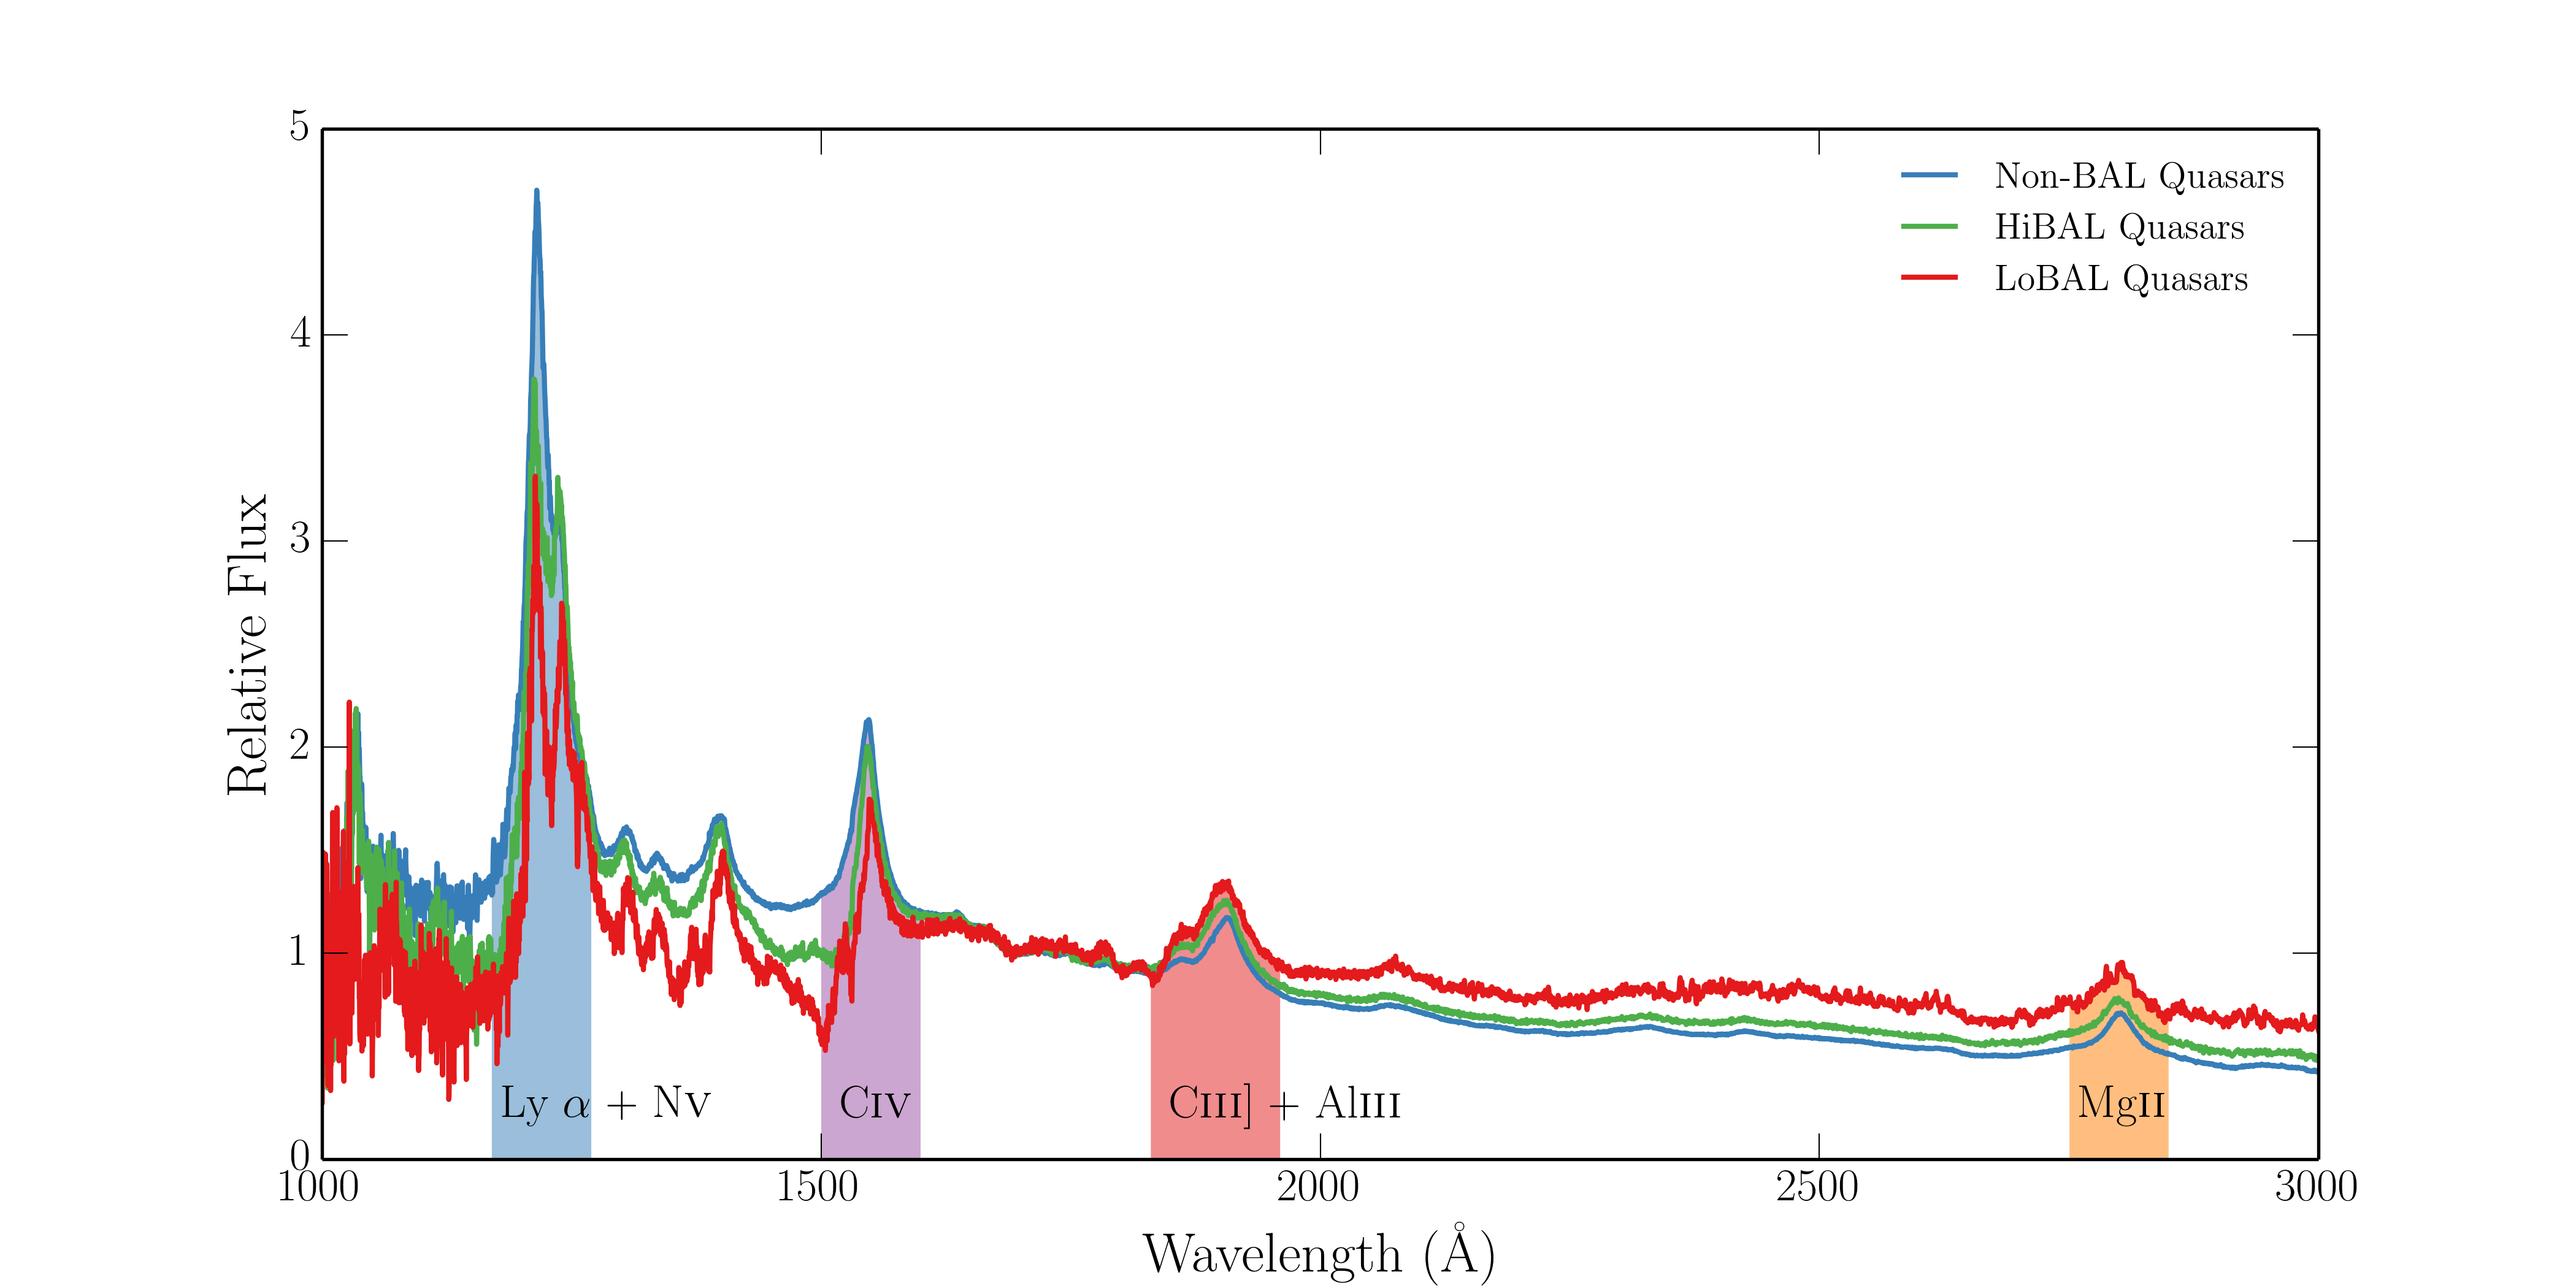
\includegraphics[width=1.0\textwidth]{figures/ewpaper/composites.png}
% \caption
% {
% SDSS Composite spectra
% }
% \label{fig:composite}
% \end{figure*} %fullpage
% The Sloan Digital Sky Survey DR7 contains ~10,000 objects in its quasar
% catalog. Many of these have been fitted with quasar templates, allowing 
% easy comparison of the equivalent width properties between the BAL and 
% non-BAL subsamples. Figure 2 shows histograms of a number of different 
% emission line properties. As found by previous authors, we find that BAL
% and non-BAL quasars really do seem to possess very similar emission line 
% properties.

% \begin{table}
% \begin{tabular}{p{2cm}p{1cm}p{1cm}p{1cm}p{1cm}}
% Sample & Redshift Range & Number of non-BAL Objects & Number of BAL objects & Number of LoBAL objects \\
% \hline \hline 
% A & $?<z<?$ & 
% \hline 
% \end{tabular}
% \caption{
% The properties of our subsamples, built from the SDSS DR7
% quasar catalog.
% }
% \label{tab:samples}
% \end{table}

\begin{figure*} %fullpage
\centering
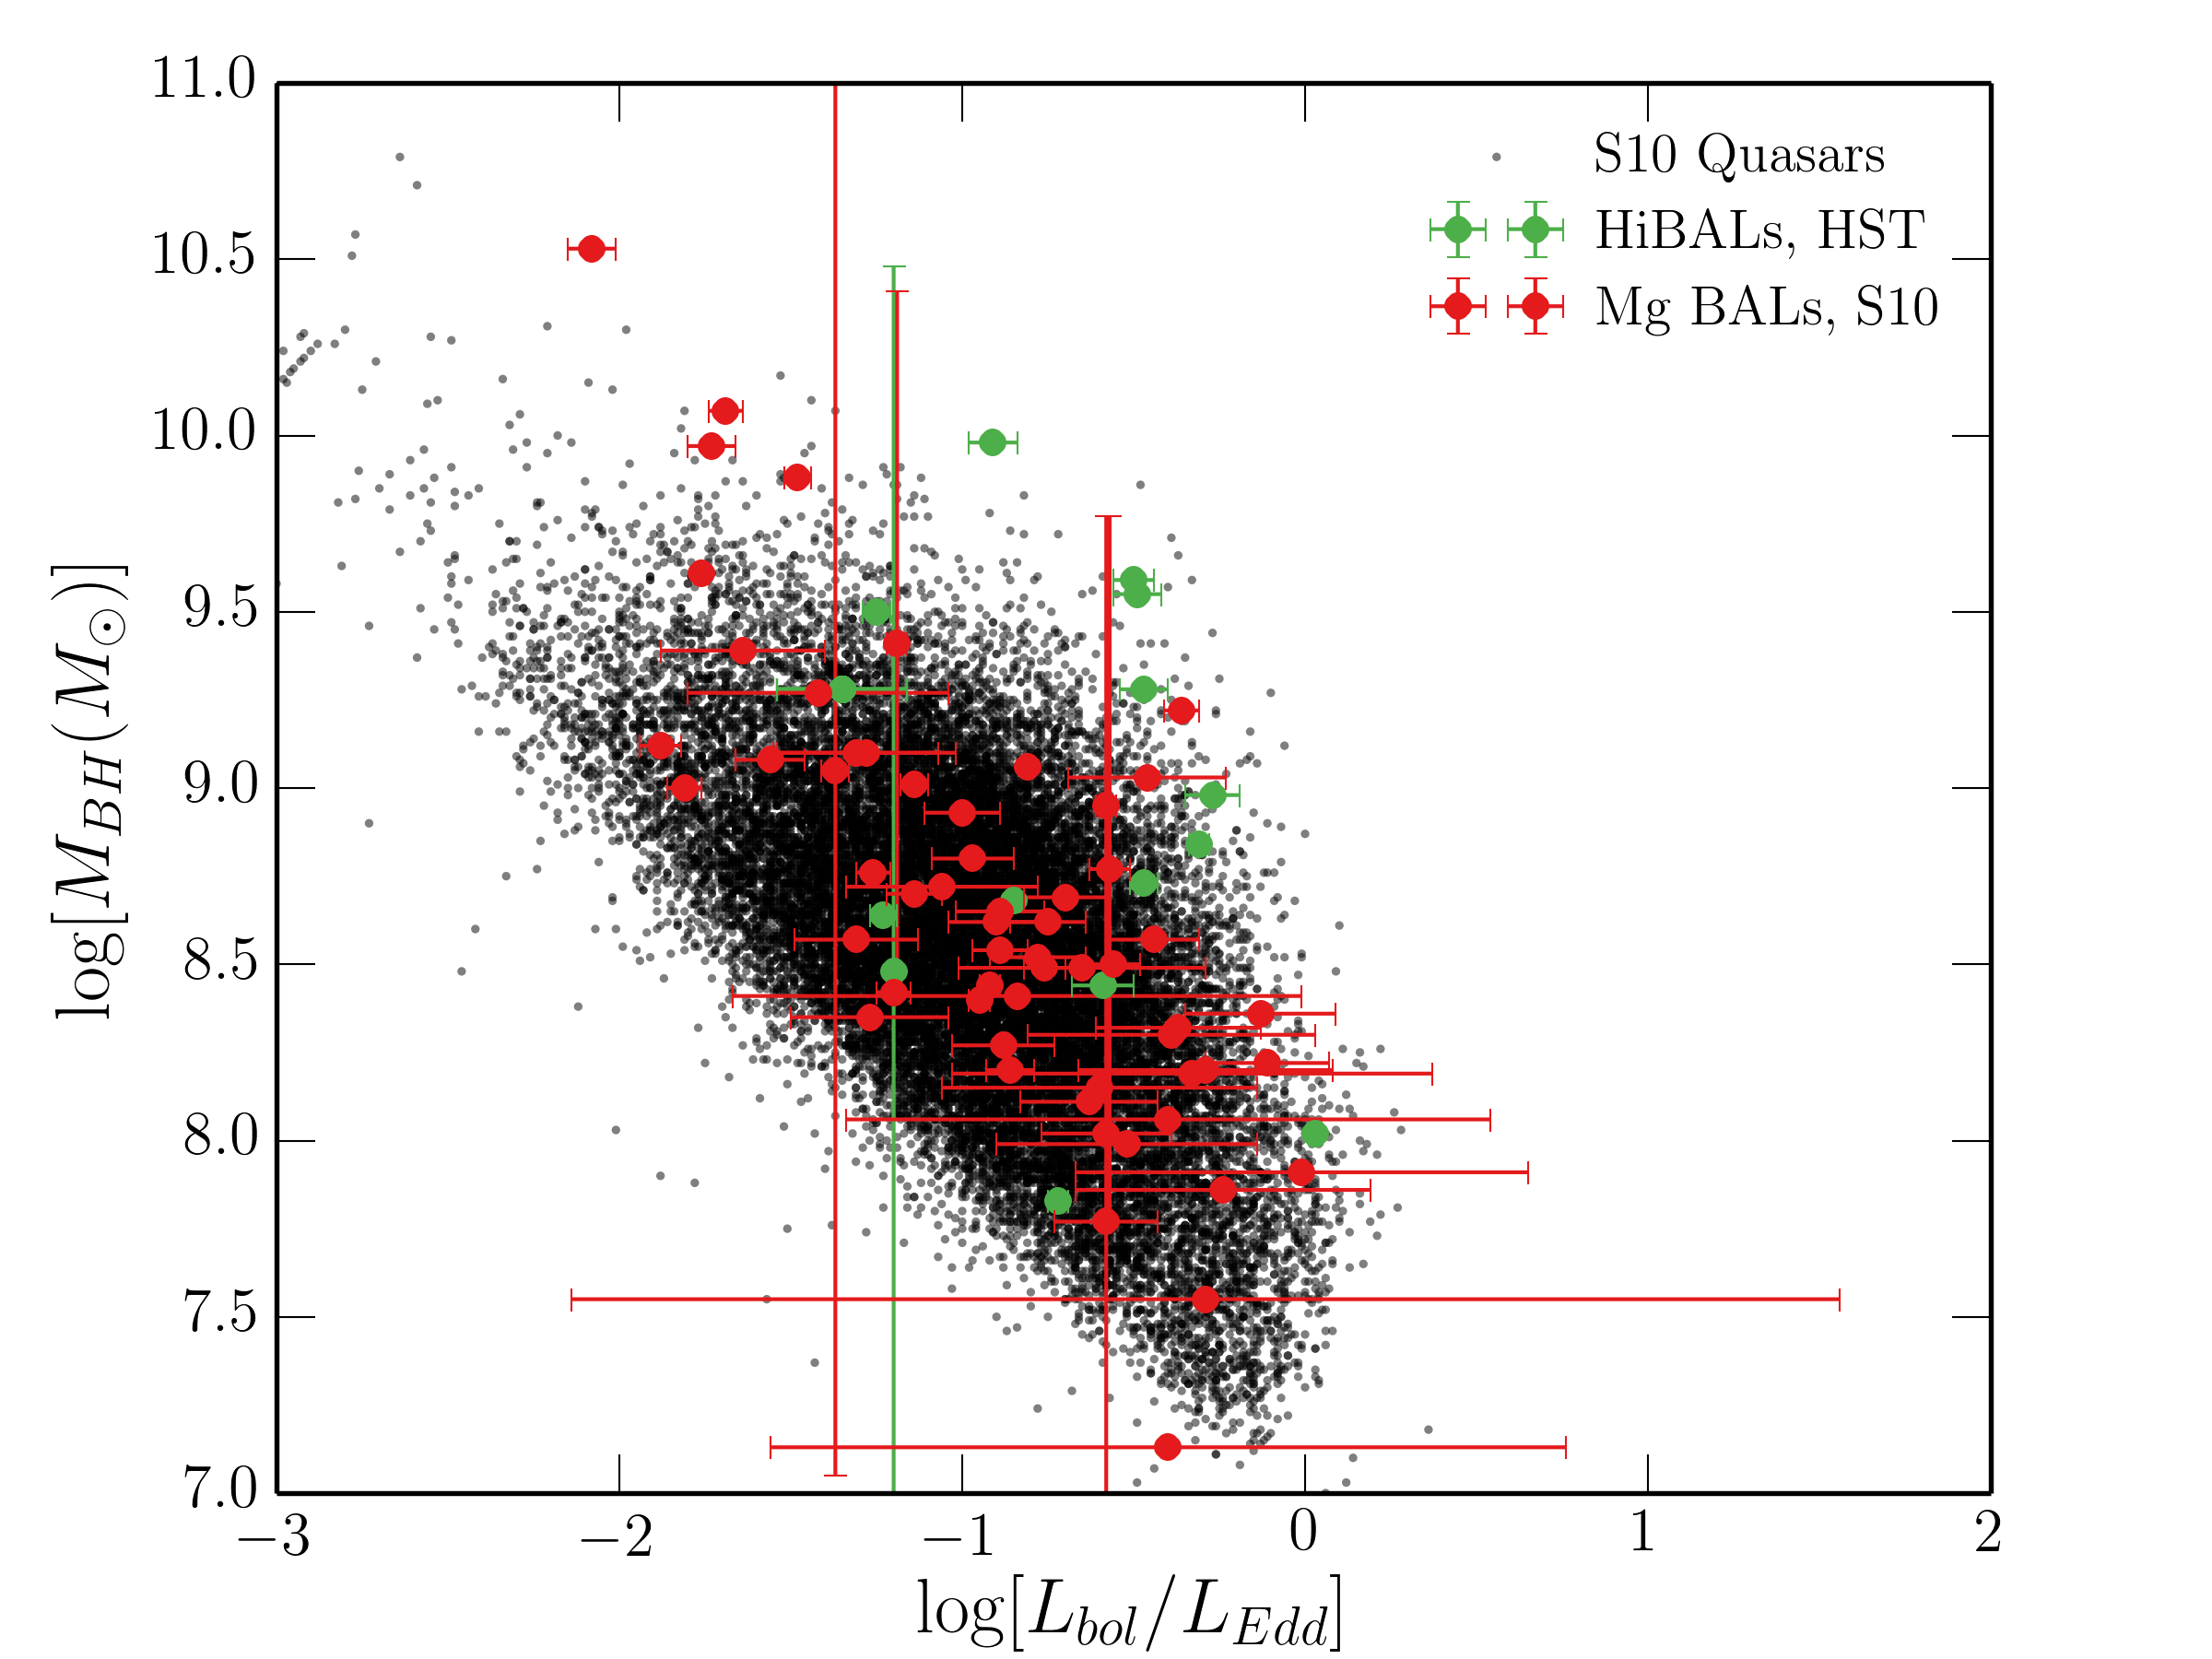
\includegraphics[width=1.0\textwidth]{figures/ewpaper/bals_scatter.png}
\caption
{
BH mass and Eddington fraction for the BAL samples plotted 
over the overall quasar sample from S11.
}
\label{fig:bal_scatter}
\end{figure*} %fullpage



\begin{figure*} %fullpage
\centering
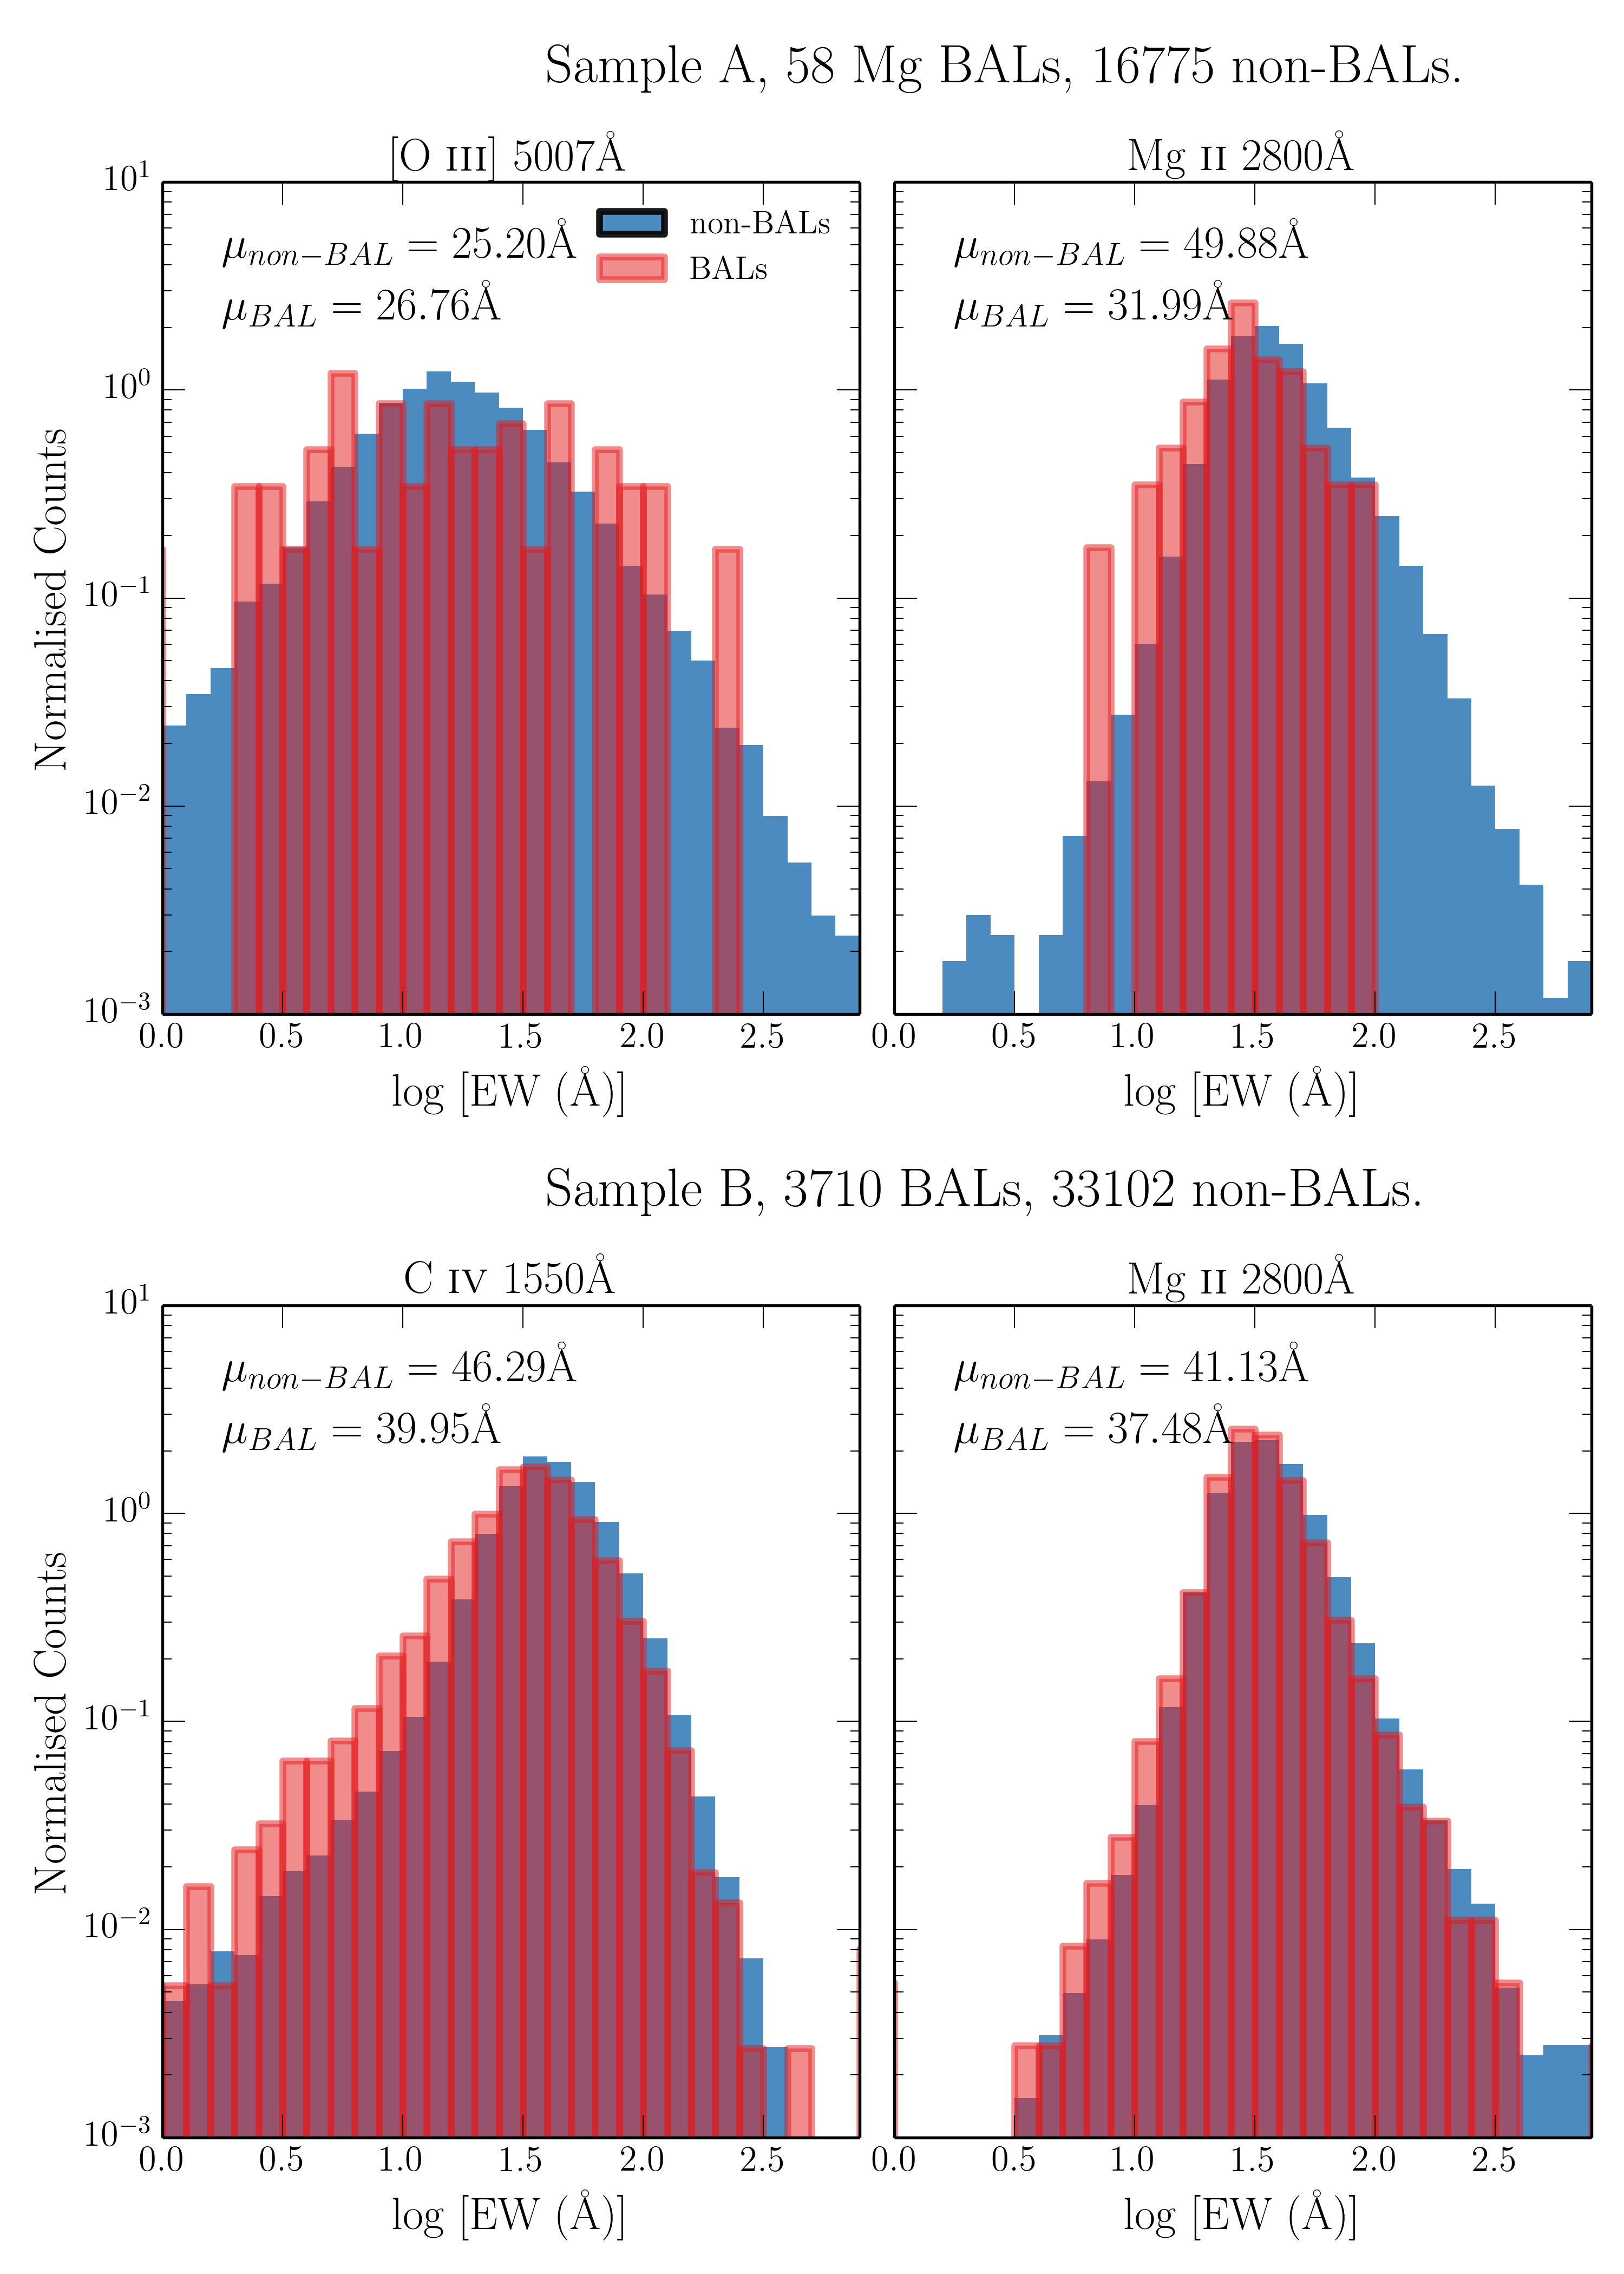
\includegraphics[width=1.0\textwidth]{figures/ewpaper/ew_hist_qsos.png}
\caption
{
Histograms of equivalent widths for three emission lines from the two different samples.
}
\label{fig:ew_hists}
\end{figure*} %fullpage

The data is sample is based upon the
\citet[][hereafter S11]{shen2011} catalog of
105,783 quasars from the The Sloan Digital Sky Survey (SDSS) 
Data Release 7 (DR7). 
As I will use emission line diagnostics in this study,
this sample must be further divided according to which 
emission lines are present in 
the SDSS wavelength range at a given redshift. 
Sample A contains all quasars within the redshift range $0.35<z<0.83$, 
such that the Mg II 2800A and \oiiifull\ line EWs are both measured, 
and Mg II BAL identification
is possible.  Sample B contains all quasars within the redshift 
range $1.45<z<2.28$, such that 
the EWs and presence of BALs in Mg II 2800A and CIV 1550A are both measurable.
The details of these samples are shown in table 1.

In attempting to draw broad conclusions about unification models as a whole,
we would like to be able to construct a large homogenous dataset of 
{\em HiBAL} and non-BAL quasars, both with \oiiifull\ EWs. Unfortunately,
the wavelength limits of SDSS do not allow this. One of the problems with
using just LoBAL quasars as tests of unification is that there is evidence 
that they are drawn from a different population than normal quasars, perhaps
suggesting an {\em evolutionary} origin. Examples include anomalously 
high LoBAL fractions in dust-reddened quasar samples \citep{urrutia2009} 
and infra-red selected samples \citep{dai2012}; 
although see also \cite{lazarova2012}.
To partially address this issue, I also build a small sample 
of HiBAL quasars in SDSS by cross-matching the S11 catalog with 
BALs identified in the HST COS archive.
BALs were selected from the COS spectra using the balnicity index, 
$BI$, defined in equation~??. HST objects were designated as HiBALS 
by satisfying the condition that $BI>0$ in one of CIV, NV, SiIV.
The mass and Eddington fraction measurements from S11, with 
errorbars, are shown against the background distribution of all quasars.

Fig. 2 shows histograms of a number of different 
emission line properties for samples A and B. 
As discussed by previous authors \cite[e.g.][]{weymann1991}, I find that BAL
and non-BAL quasars really do seem to possess very similar emission line 
properties. The EW is related to the `face-on' equivalent width,
$EW_0$ by the equation
\begin{equation}
\ew = \ew_0 /~\epsilon(\theta)
\end{equation}
where $\theta$ is the viewing angle with respect to the symmetry axis 
and $\epsilon(\theta)$ is the `angular emissivity function', which describes 
how the continuum luminosity from the disc varies as a function of viewing angle.
For a foreshortened disc this is simply $\epsilon(\theta) = \cos \theta$.

Thus, if BAL quasars are viewed from a larger viewing angle on average then one
would expect them to possess higher EWs, with a broader distribution.
It is already apparent from figure 1 that the BAL distribution mean 
is not systematically higher than the non-BAL
mean -- in fact, it is lower. This is not expected from a model
in which the continuum is foreshortened and BAL outflows are at all equatorial.
This problem is examined further in section~\ref{sec:mc_angular}. 
First, I will examine the motivations for different forms of \ept\ 
in AGN and quasars.

\section{The Angular Distribution of Emission from an Accretion Disc}
\label{sec:disc_agn}

\noindent 
The most widely-used theoretical model for an accretion disc
was proposed by Shakura \& Sunyaev (1973; hereafter SS73). 
\nocite{shakurasunyaev1973}
There are a number of well-documented problems when fitting 
AGN SEDs with SS73 accretion disc models (REFs), and there are also 
tensions with the `accretion disc size' relation from time lags \citep{edelson2015}
and microlensing \citep{morgan2010}. Despite these problems, 
\cite{capellupo2015} recently had 
some success fitting VLT XSHOOTER spectra of AGN when the effects of
GR, mass-loss and comptonisation were included.
In this section, I start by discussing the angular distribution of
emission from an SS73 disc, before discussing opacity and GR 
effects. In order to explore these effects, I use \agn\
\citep{hubeny2000,davishubeny2006,davis2007}. I stress that the 
discussion here is not limited to SS73 discs; the only real condition
for the expected angular distributions derived here is that the 
disc is geometrically thin and optically thick.

\subsection{Standard Thin Disc Models}

\noindent
Any geometrically thin, optically thick disc will appear
foreshortened and limb darkened (if temperature decreases
with height from the central disc plane). 
Foreshortening is a simple $\cos \theta$ geometric effect, 
where $\theta$ is the inclination with respect to the vertical z axis, which
is perpendicular to the disc plane.
Limb darkening, $\eta(\theta)$, is given by
\begin{equation}
\eta(\theta) = a \left( 1 + b \cos \theta \right),
\end{equation}
where $a$ is a normalisation constant and $b$ governs the strength
of the limb darkening. $b=3/2$, known as the Eddington approximation
tends to given good agreement with solar observations 
\citep[e.g.][]{mihalas}. The two effects can be 
combined to give an angular emissivity function, of
\begin{equation}
\epsilon(\theta) = a \cos \theta \left( 1 + \frac{3}{2} \cos \theta \right).
\end{equation}

\subsection{Including GR, Comptonisation and Opacity Effects}

\noindent
In reality, limb darkening is not frequency independent and 
depends on the bound-free and bound-bound opacities in the disc.
In addition, it has been shown that GR can `isotropize' the radiation
field in XRBs \citep{zhang1997,munozdarias2013}, in some cases overcoming
foreshortening effects. To assess the impact of GR and disc opacities
on \ept\ I use \agn\ models, which uses stellar atmosphere 
calculations to calculate the 
SED in a series of annuli, before using the \kerrtrans\ code 
to calculate the emergent SED by ray-tracing along Kerr geodesics.
Fig.~\ref{fig:agnspec_disc} shows \ept\ as a function of 
$\theta$ for \agn\ models for minimally and maximally spinning BHs,
compared to foreshortened and limb-darkened predictions for SS73 models.
Clearly, there is very little effect; 
the accretion disc is still strongly anisotropic in the relevant wavebands.

\begin{figure}
\centering
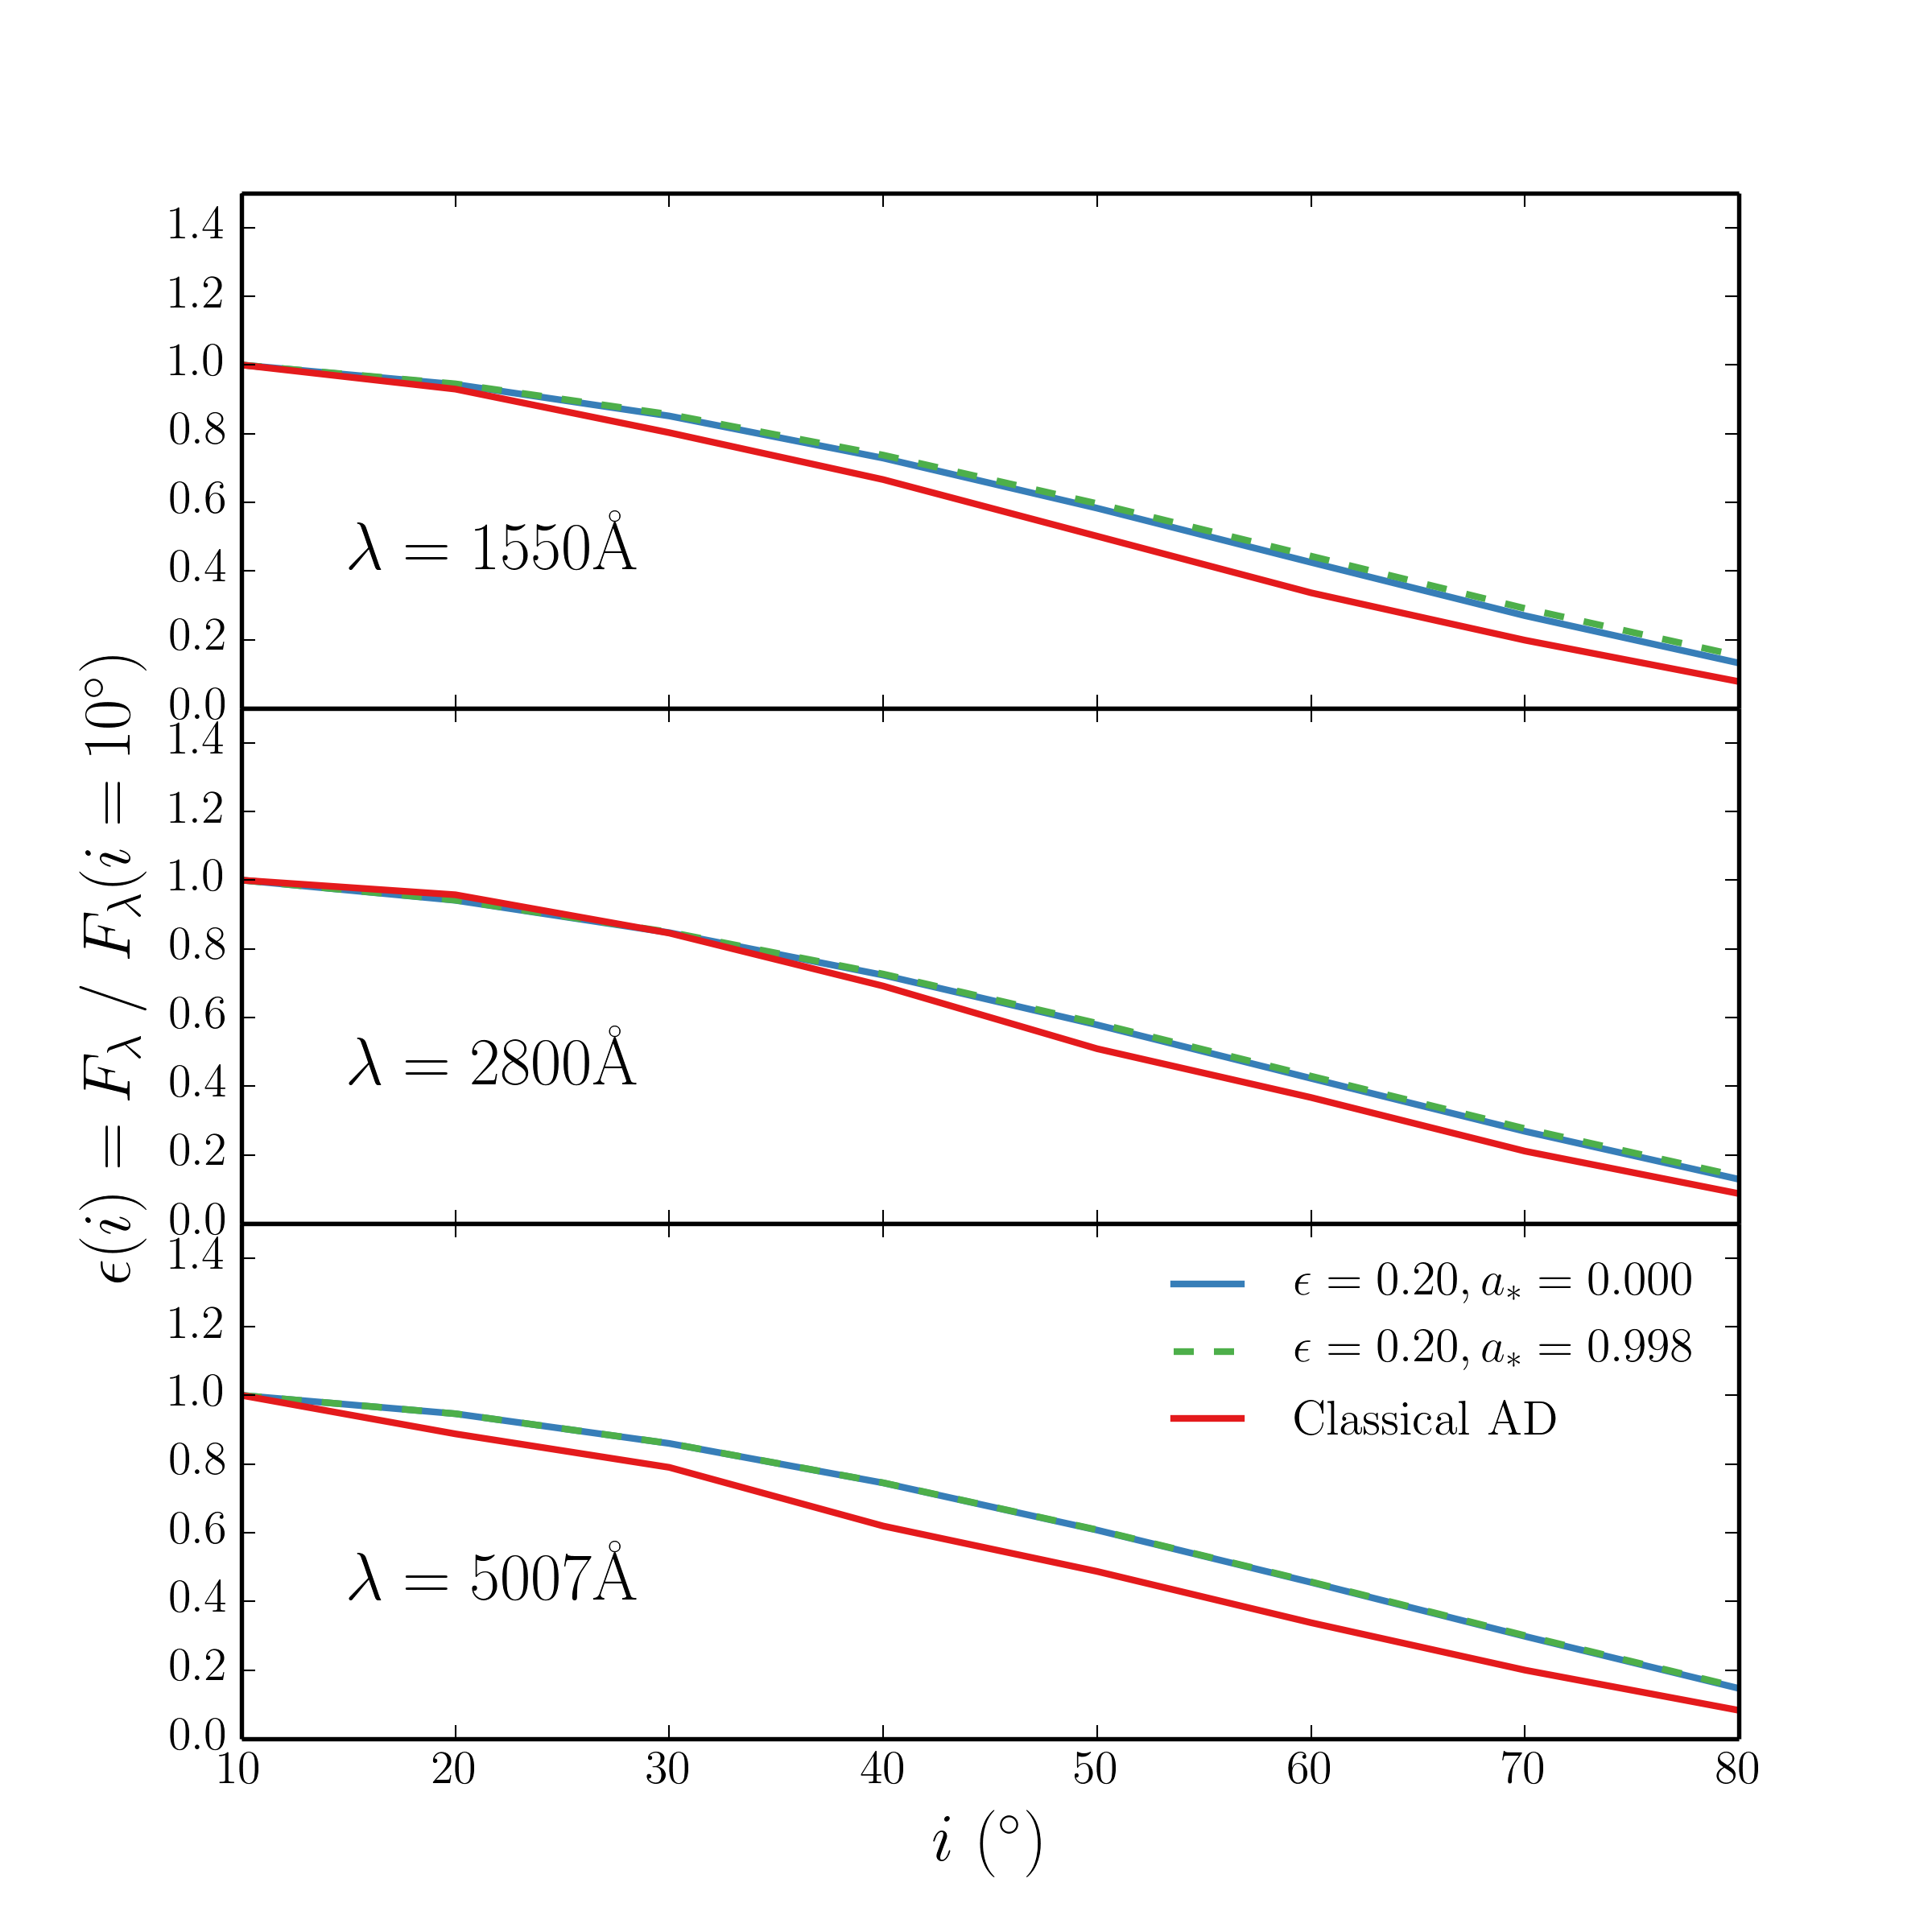
\includegraphics[width=1.0\textwidth]{figures/ewpaper/agnspec.png}
\caption
{
Monochromatic continuum luminosities from AGNSPEC and classical thin disc
models.
}
\label{fig:agnspec_disc}
\end{figure} 
% Including GR, Comptonisation and Opacity Effects

% \subsection{Alternative Continuum Models: Irradiation and Truncated Discs}

% Alternative Models exist...






\section{Predicted EW distributions compared to observations: A Monte Carlo approach}
\label{sec:mc_angular}

\begin{figure}
\centering
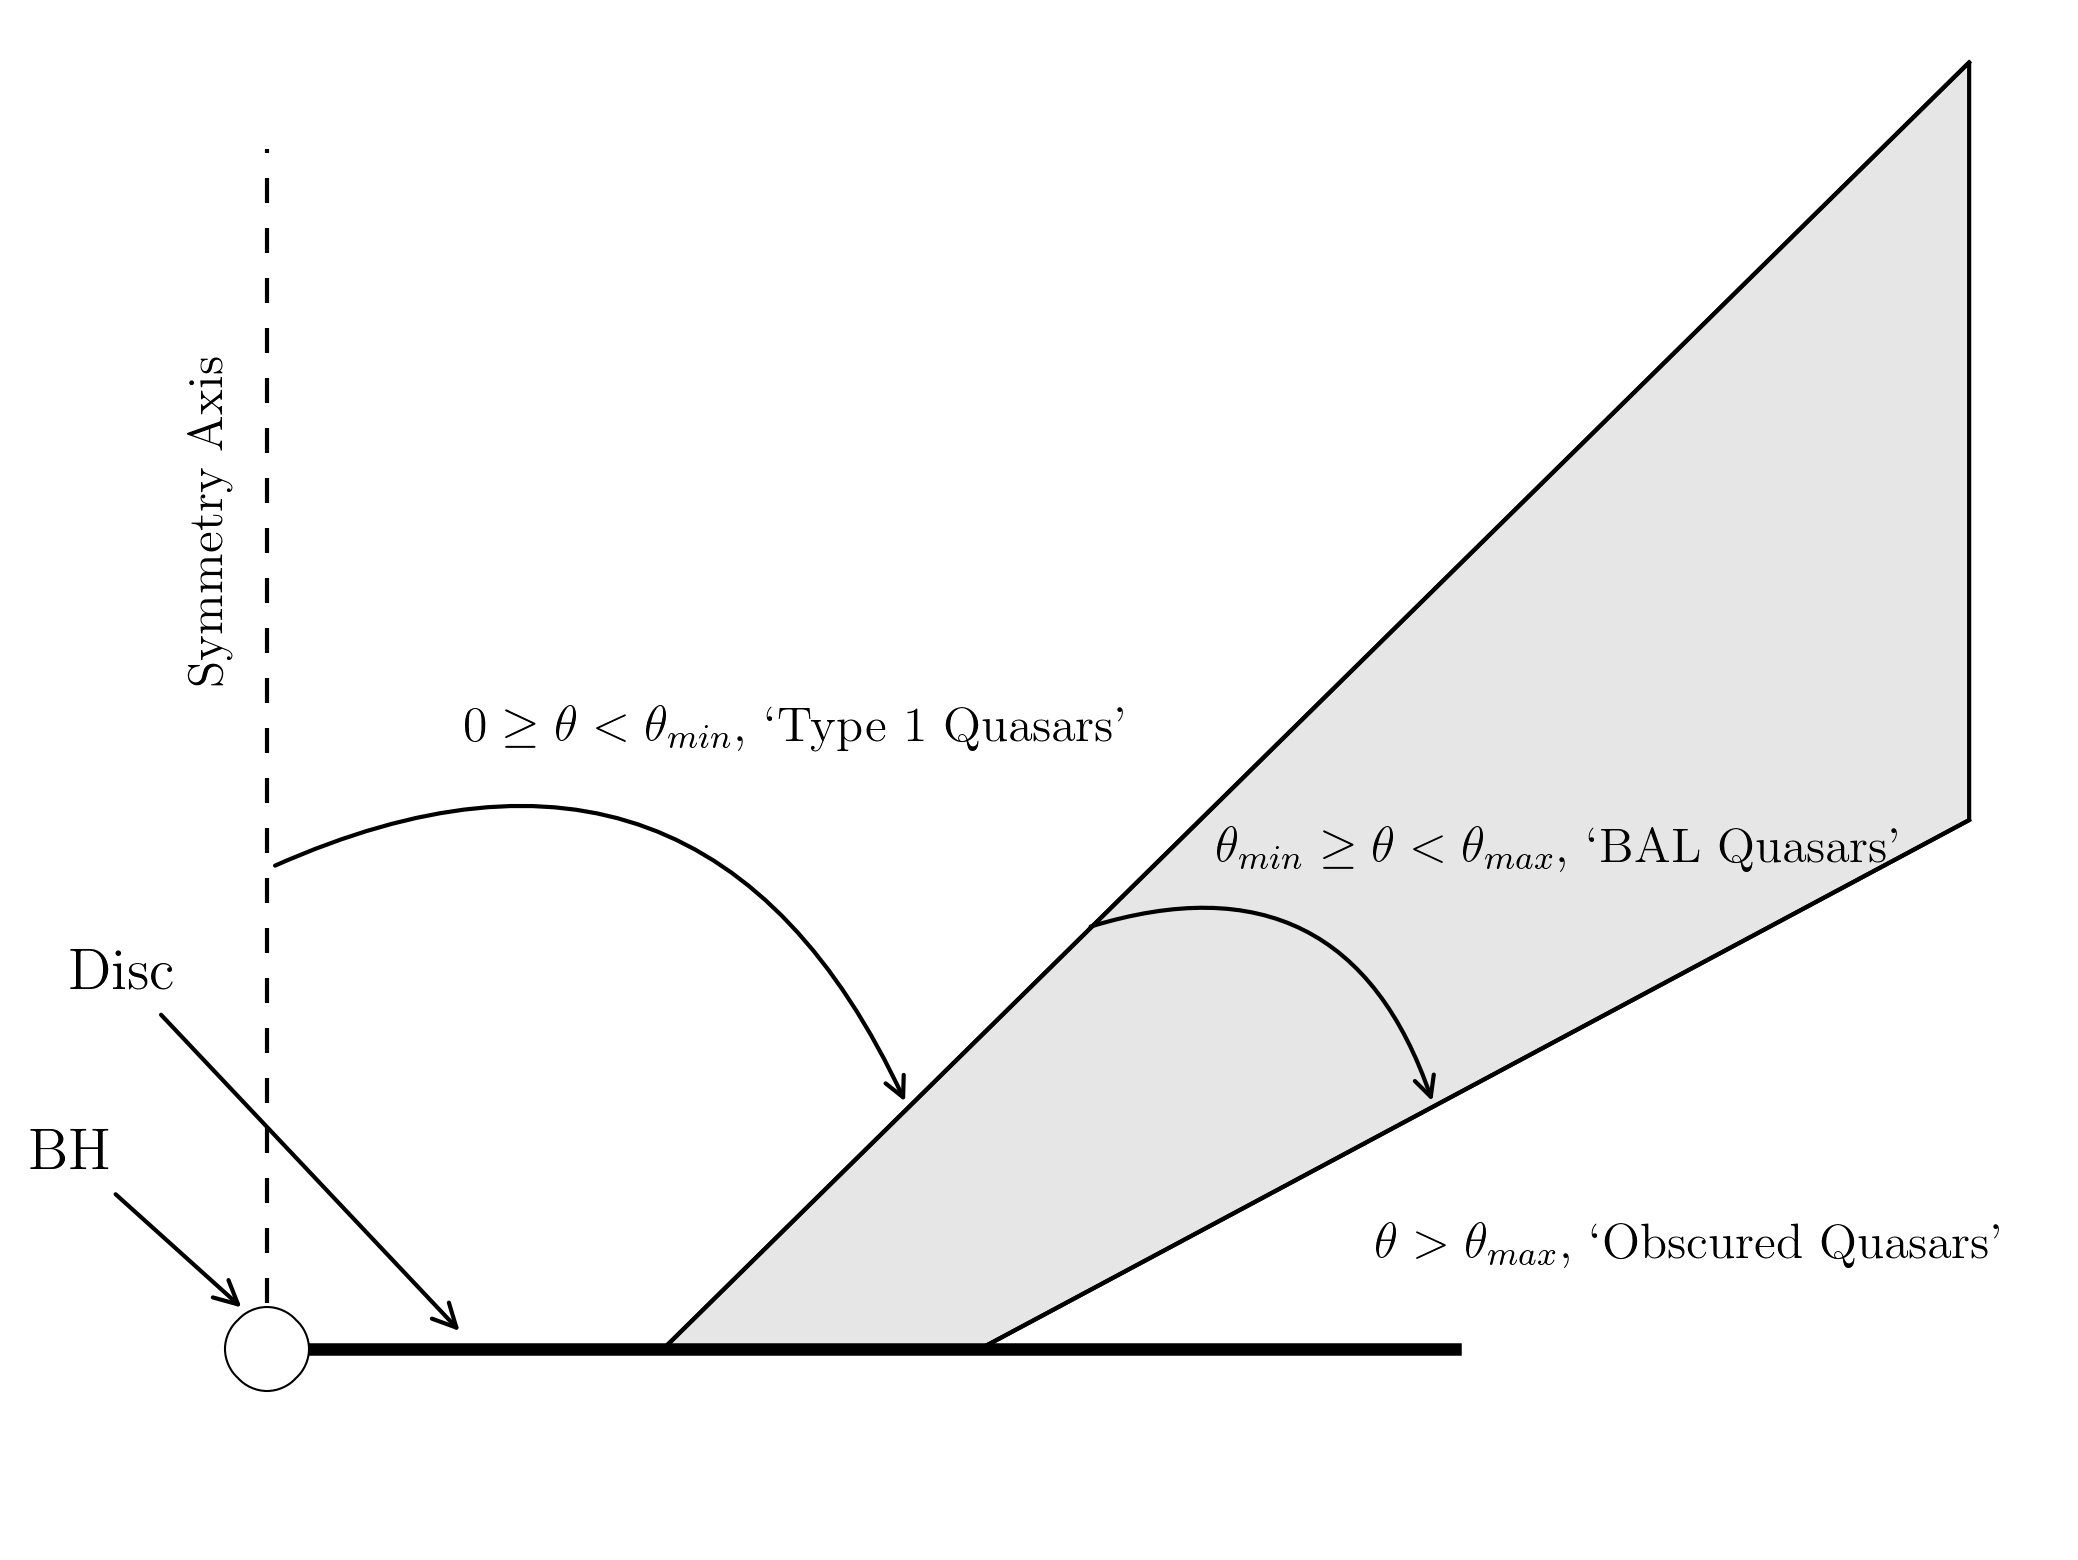
\includegraphics[width=1.0\textwidth]{figures/ewpaper/fig2_cartoon.png}
\caption
{
The geometry of the toy model used to carry out the Monte Carlo simulations
}
\label{fig:cartoon}
\end{figure}


I assume $\epsilon(\theta) = \cos \theta$, as this is the conservative estimate. 
% Unfortunately, it is very difficult to construct an intrinsic `face-on' distribution
% of EWs in quasars. This is mainly because the intrinsic face-on luminosities
% and inclination distribution of the systems is not known, meaning that deconvolving
% these effects is challenging. If an intrinsic, face-on distribution could be constructed
% then models of continuum emission could be used to derive predicted EW distributions
% for a grid of outflow geometries. These predicted distributions could then be compared 
% to the observed distributions and constraints placed on BAL viewing angles via,
% e.g., a Kologomorov-Smirnov test. Despite these difficulties, it is still relatively easy to 
% demonstrate that the EW distribution
% in BAL quasars is not well produced by a model in which the accretion disc is foreshortened 
% and BAL quasars are viewed from high inclinations. We will show this by first qualitatively
% examining the effect of inclination on a log-normal distribution of EWs, before conducting
% a simple Monte Carlo experiment to ascertain which geometries best reproduce the observed
% distributions.

% \subsection{The Effect of Inclination on a Log-normal EW distribution}

% Fig.~\ref{fig:ew_cartoon} shows the effect of different viewing angles 
% for BAL and non-BAL quasars for four different geometries. In each case, the
% intrinsic EW distribution, $g({\rm EW})$ is taken to be a normal
% distribution with $\mu=10$\AA and $\sigma=5\AA$. 
% We then choose $10^6$ isotropic angles on the sky and apply a 
% flux selection effect, and designate each of the angles that passes the selection 
% criteria as a BAL or non-BAL viewing angle. We assume
% $\epsilon(\theta) = \cos \theta$, as this is the conservative estimate. 
% Viewing BALs from high inclinations results in both a systematic shift in the mean to
% higher EWs, as well as a broader distribution, with the characteristic tail at 
% extreme inclinations. 

% \begin{figure*} %fullpage
% \centering
% 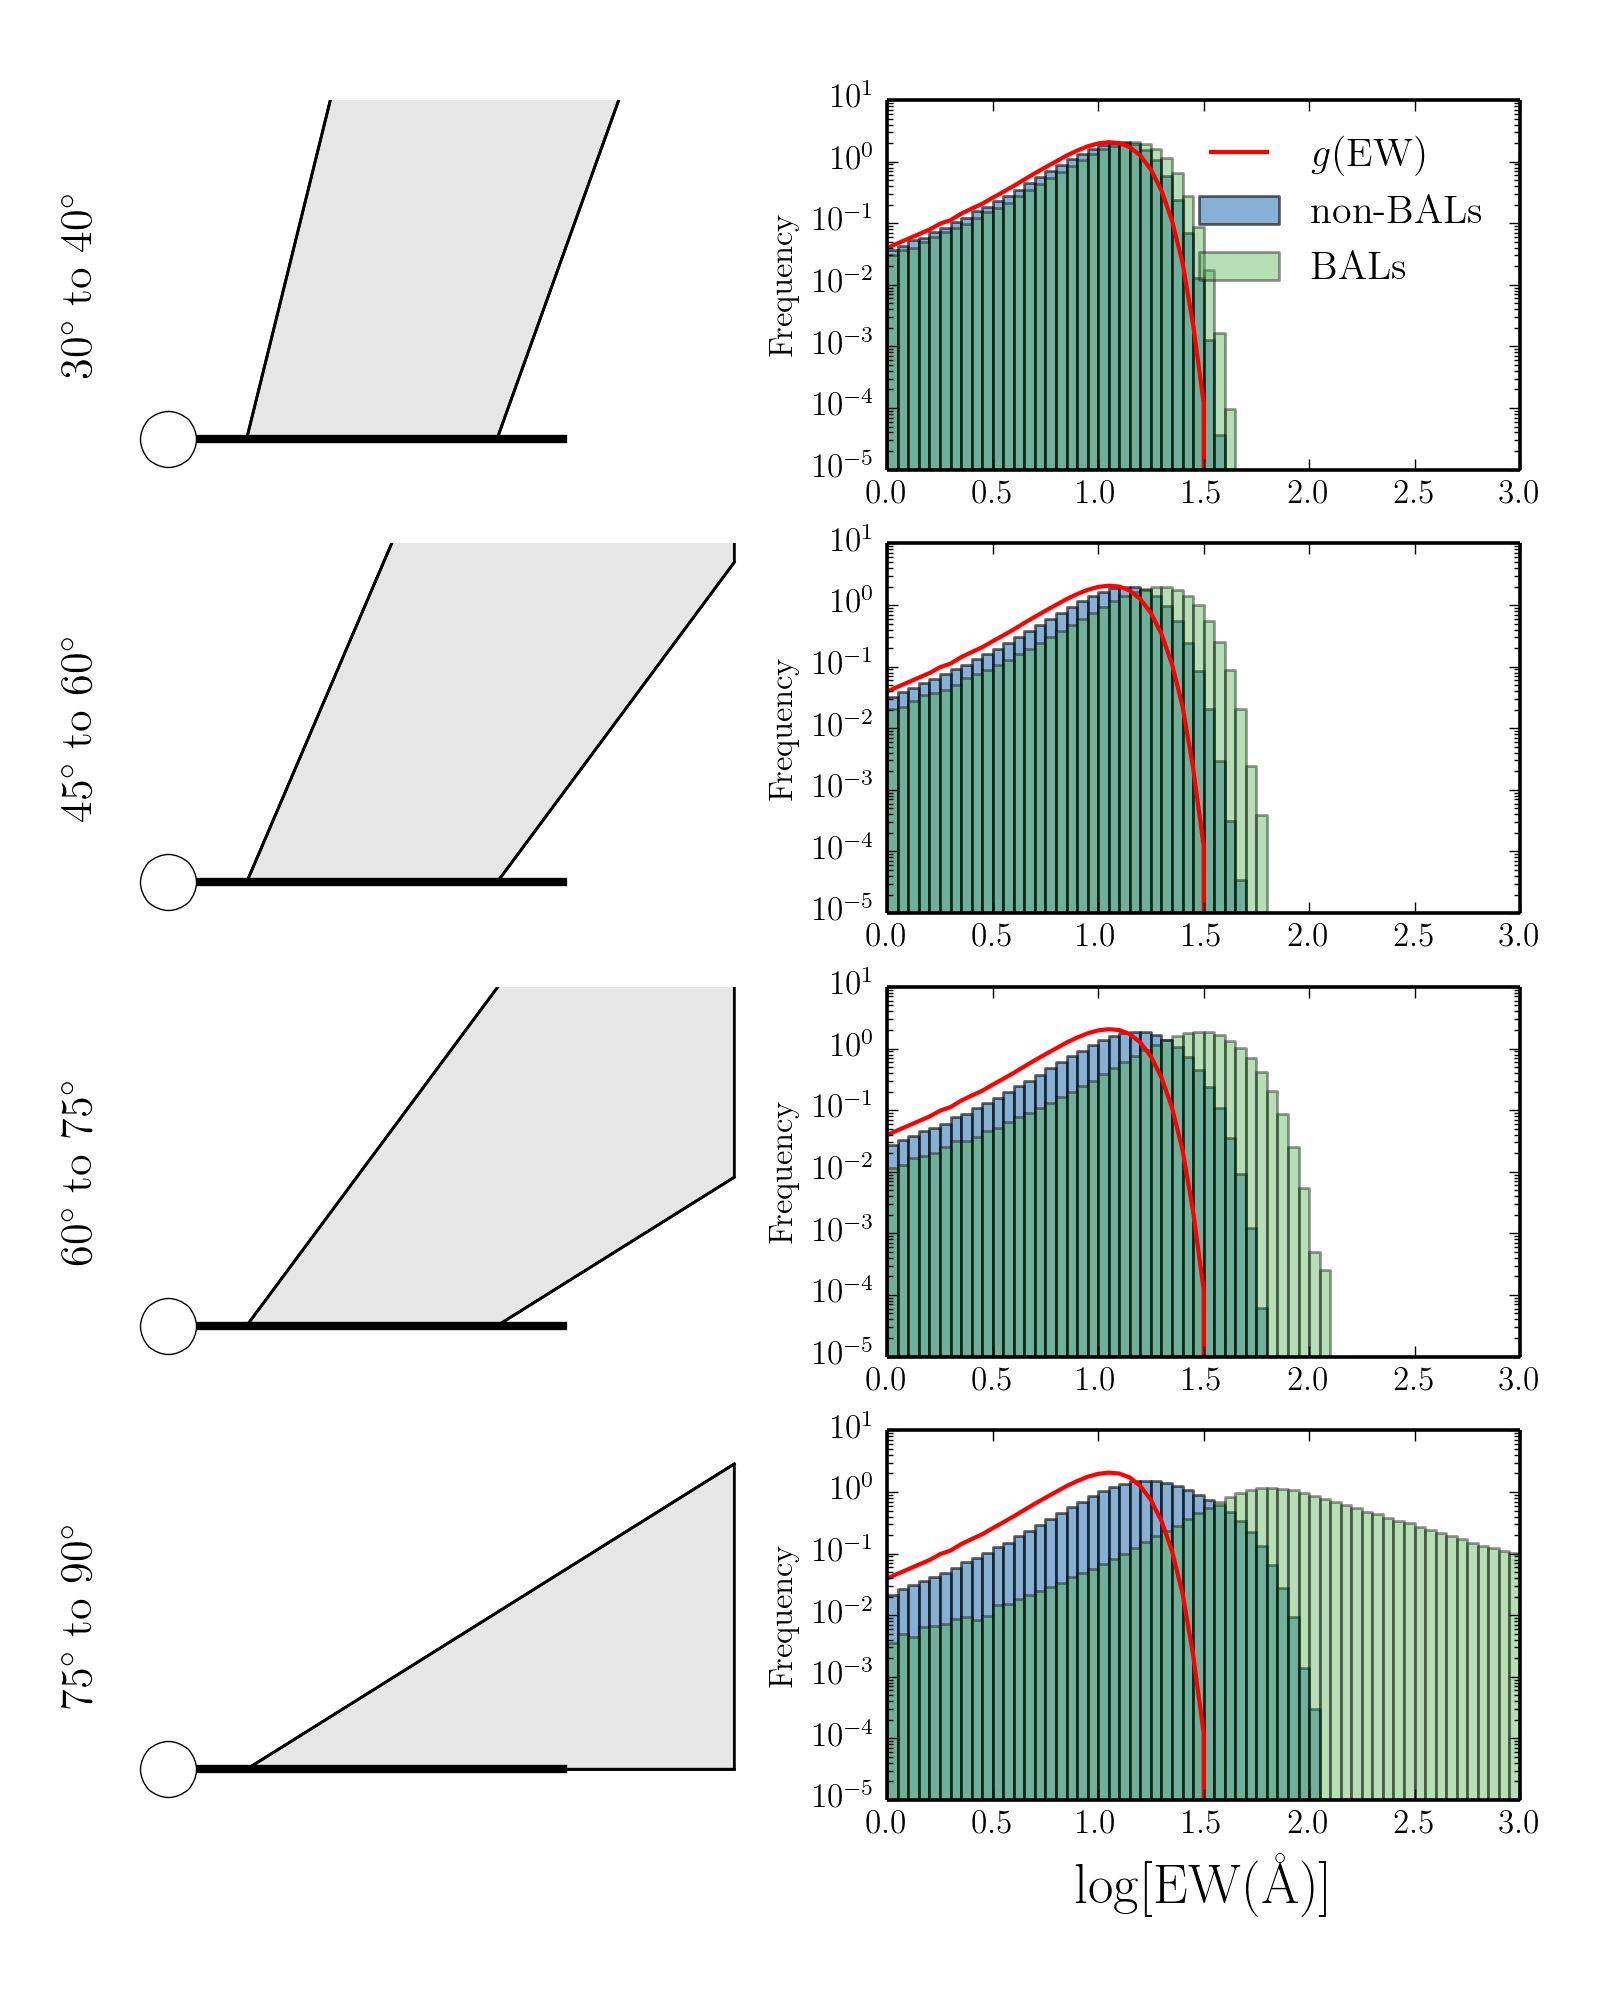
\includegraphics[width=1.0\textwidth]{figures/ewpaper/ew_with_cartoon.png}
% \caption
% {
% Histograms of equivalent widths for BAL and non-BAL quasars for a number of
% different toy unification geometries.
% }
% \label{fig:ew_cartoon}
% \end{figure*} %fullpage

% \subsection{Monte Carlo Approach}

\begin{figure*} %fullpage
\centering
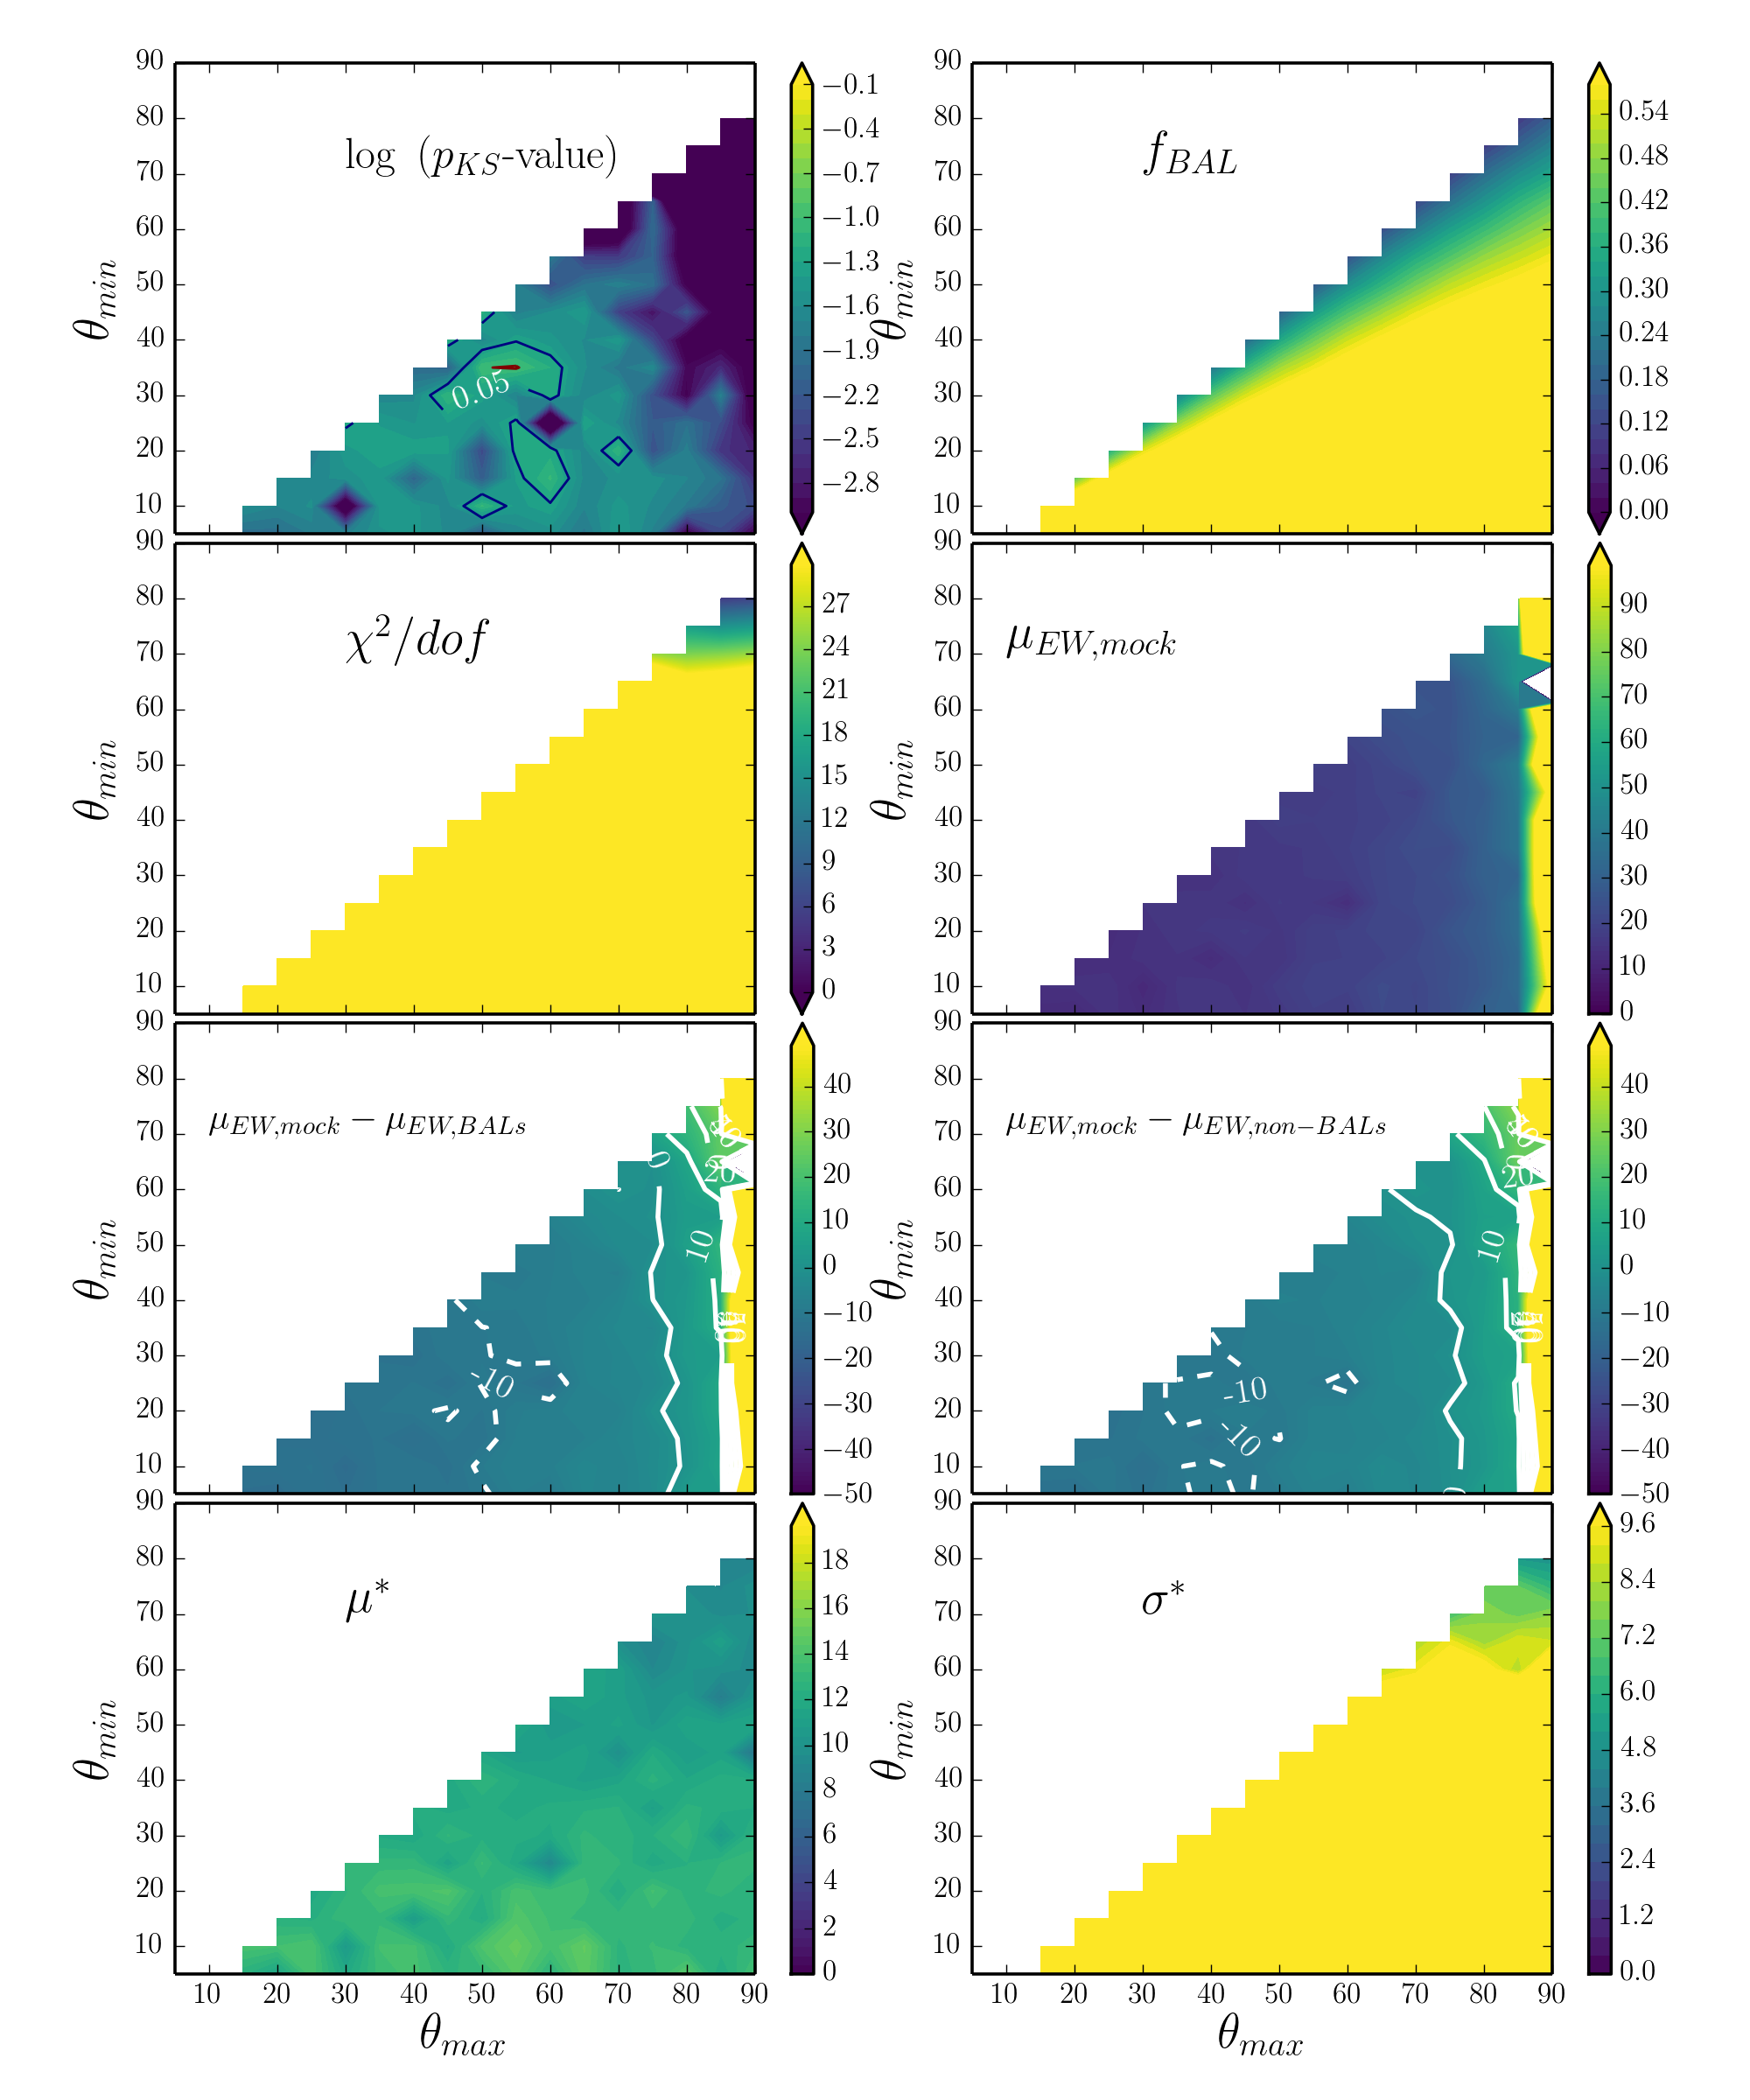
\includegraphics[width=1.0\textwidth]{figures/ewpaper/four_ew_o3_max_sdss.png}
\caption
{
Contour plots from the Monte Carlo simulations.
}
\label{fig:contour}
\end{figure*} %fullpage

The Monte Carlo simulation undergoes the following steps:

\begin{enumerate}
	\setlength\itemsep{1em}
	\item A set of isotropic angles is chosen such that $P(\theta)\propto d\Omega(\theta)$.
	If $\theta_{min}<\theta<\theta_{max}$ then the fake object is flagged as a mock BAL. 
	If $\theta<\theta_{min}$ then the fake object is designated a non-BAL, and otherwise
	the object is ignored. To be included in the sample, the object also has to 
	survive a selection test based on a arbritrary flux selection limit, to simulate the
	distribution of angles in a flux-limited sample.
	\item I then construct a best estimate of the intrinsic (i.e. `face-on')
	EW distribution for non-BAL quasars. This is done via a $\chi^2$ minimisation,
	by finding the gaussian with $\mu$ and $\sigma$ which best 
	reproduces the observed distribution when convolved with
	the non-BAL angles generated in the previous step. 
	a $\chi^2$ minimisation.
	\item For each mock sample, a EW$_0$ is drawn from the intrinsic gaussian.
	\item A mock EW is estimated such that $\ew = EW_0 / \epsilon(\theta)$,
	and this process is repeated to build up a mock sample of objects.
	\item The number of objects in the mock sample with 
	$\theta_{min}<\theta<\theta_{max}$ is recorded, providing an 
	estimate of the expected BAL fraction for this wind geometry. 
	This already includes a selection effect for the weaker continuum flux.
	\item The value of the K-S test statistic is recorded, in which the 
	mock BAL sample is compared to the real BAL sample. The 
	mean and variance of the mock sample is also recorded. 
	This allows us to ascertain which regions
	of parameter space best fit the observed BAL distribution
\end{enumerate}

This process is repeated for a grid of $\theta_{min}$ and $\theta_{max}$. The 
results are shown in figure~\ref{fig:contour}, in which the mean, 
standard deviation and $f_{BAL}$ are shown as a function of $\theta_{min}$ 
and $\theta_{max}$. As expected, equatorial viewing angles are strongly 
disfavoured. 



% \subsection{Favoured Geometries}

% The methods above imply that we favour blah.

% \section{The Angular Distribution of Line Emission}

% {\color{blue}
% Angular distribution of line emission derivations,
% showing in what limits emission lines will have the same
% angular emissivity distribution as an accretion disc.
% }

% \bigskip

% \label{lines}
% Here we consider three geometries for BLR emission regions. The first is
% a spherical, cloud-like structure with no velocity gradients. 
% The second is a disc structure with Keplerian velocity components, 
% potentially with the addition of outflowing material. the third is a 
% disc-like geometry with turbulent velocity gradients.

% Optically thin line emission is always isotropic in the rest frame
% of the emitting plasma. Optically thick line emission will have an angular
% emissivity function that varies according to the geometry of the 
% emitting region and the velocity gradients present. 
% We can thus use Sobolev
% theory to derive the angular emissivity function for
% line emission. Invoking the Sobolev approximation, we can write the 
% optical depth in a non-monotonic velocity field as

% \begin{equation}
% \tau = \frac{\kappa~\rho~\sigma}{| \mathbf{\hat{n} \cdot \Lambda \cdot \hat{n} |}}
% \end{equation}

% And following \cite{MCGV95} we can derive an expression for $Q=|\mathbf{\hat{n}\cdot\Lambda \cdot\hat{n}}|$

% \begin{equation}
% Q = x
% \end{equation}


% Following \cite{hornemarsh1986} and \cite{horne1995}, we can write the line optical depth as
% \begin{equation}
% \tau_\nu = \tau_0 \exp \left[ - \frac{1}{2} 
% \left( \frac{V - V_0}{\Delta V} \right)^2 \right],
% \end{equation}
% where $\tau_0$ is the line centre optical depth given by
% \begin{equation}
% \tau_0 = \frac{W}{}
% \end{equation}


\section{Discussion}
\label{sec:discuss_ew}
I have demonstrated that the EW distributions of the 
\oiiifull\ emission line in quasars is not consistent with a 
model in which BAL quasars are viewed from equatorial angles 
and the continuum emission originates from
a foreshortened accretion disc. This conclusion would be strengthened were 
I to include limb darkening. This conclusion is extendible to the broad 
emission lines, with the caveat that those lines are dipole 
transitions and so opacity effects can change the angular distribution of 
emission. I will now explore how the above results compare to other
observations of quasars that are expected to probe system orientation.

\subsection{Eigenvector 1}

\begin{table}
\centering
\begin{tabular}{p{2cm}p{2cm}p{2cm}p{2cm}}
\hline Par. A & Par. B & $r_{corr,AB}$ (non-BALs) & $r_{corr,AB}$ (BALs) \\ 
\hline \hline 
$\log$[\ewo] & \fwh\ & 0.14 & 0.18 \\
$\log$[\ewo] & $R_{{\rm Fe \textsc{ii}}}$ & $-0.51$ & $-0.67$ \\
\fwh\ & $R_{{\rm Fe \textsc{ii}}}$ & $-0.26$ & $-0.42$ \\
\end{tabular}
\centering
\caption
[Eigenvector 1 correlation coefficients]
{
Eigenvector 1 correlation coefficients
}
\label{ev1_corr}
\end{table}

Eigenvector 1 (EV1) is a fundamental parameter space for AGN and quasars
\citep{borosongreen,sulentic2000ev1,marziani2001,shenho2014}. 
It relates the 
FWHM of \hb, \fwh, the relative iron strength, 
$R_{{\rm Fe \textsc{ii}}}$ and
the \ewo. Both \ewo\ and \fwh\ have been used as orientation
indicators, and so comparing the BAL EV1 distribution to the non-BAL EV1 
distribution is particularly interesting. 

Fig.~\ref{fig:bal_ev1} shows the quasar distribution from sample A 
in EV1 parameter space, with BAL quasars from samples A and B overplotted.
\cite[][hereafter SH14]{shenho2014} propose 
that the main inclination driver in the parameter space
is \fwh, and that high inclination sources should thus cluster around
a diagonal line from the lower right to upper left quadrants. Conversely,
R11's analysis instead suggests that high inclination sources should cluster
around high EW OIII widths. As \ewo\ and \fwh\ are very weakly correlated
(Spearman's rank coefficient of 0.13), this means they should lie to
the left of the parameter space. Inspection of the figure clearly 
shows that BAL quasars are not only found in one region of the 
EV1 parameter space. 

In order to assess this more quantitavely, I have shown contours of 
quasar counts overlaid on the scatter plot. The contours correspond
to the number of objects in each bin, where the bins are of size
$\Delta R_{{\rm Fe \textsc{ii}}} = 0.2$ and $\Delta$\fwh$=500$km~s$^{-1}$.
The percentage of quasars falling within the inner contour is 45\%, 
whereas only 18\% of BAL quasars fall in the space. Conversely, 24\% 
of BAL quasars fall outside the outermost contour compared to 10\% of 
non-BAL quasars. It would therefore appear that BAL 
quasars are preferentially clustered towards the high-mass and 
high-inclination end of EV1 space (under the interpretation of SH14).
This is further illustrated by Fig.~\ref{fig:bal_ev1_bins},
which shows the LoBAL fraction in the same bins, compared to the 
mean LoBAL fraction. This is again suggestive of an overdensity 
towards the upper right of the parameter space.
It is also clear that a unification picture in which BAL 
quasars are viewed exclusively from high inclinations is ruled out,
under both the R11 and SH14 interpretations. 

Larger datasets, preferably including HiBAL quasars with EV1 measurements, 
are needed in order to properly constrain the EV1 behaviour of BAL quasars.
However, overall, the behaviour of \fwh\ strengthens the above 
conclusion that BAL quasars are not always viewed from 
extreme inclinations.

\begin{figure}
\centering
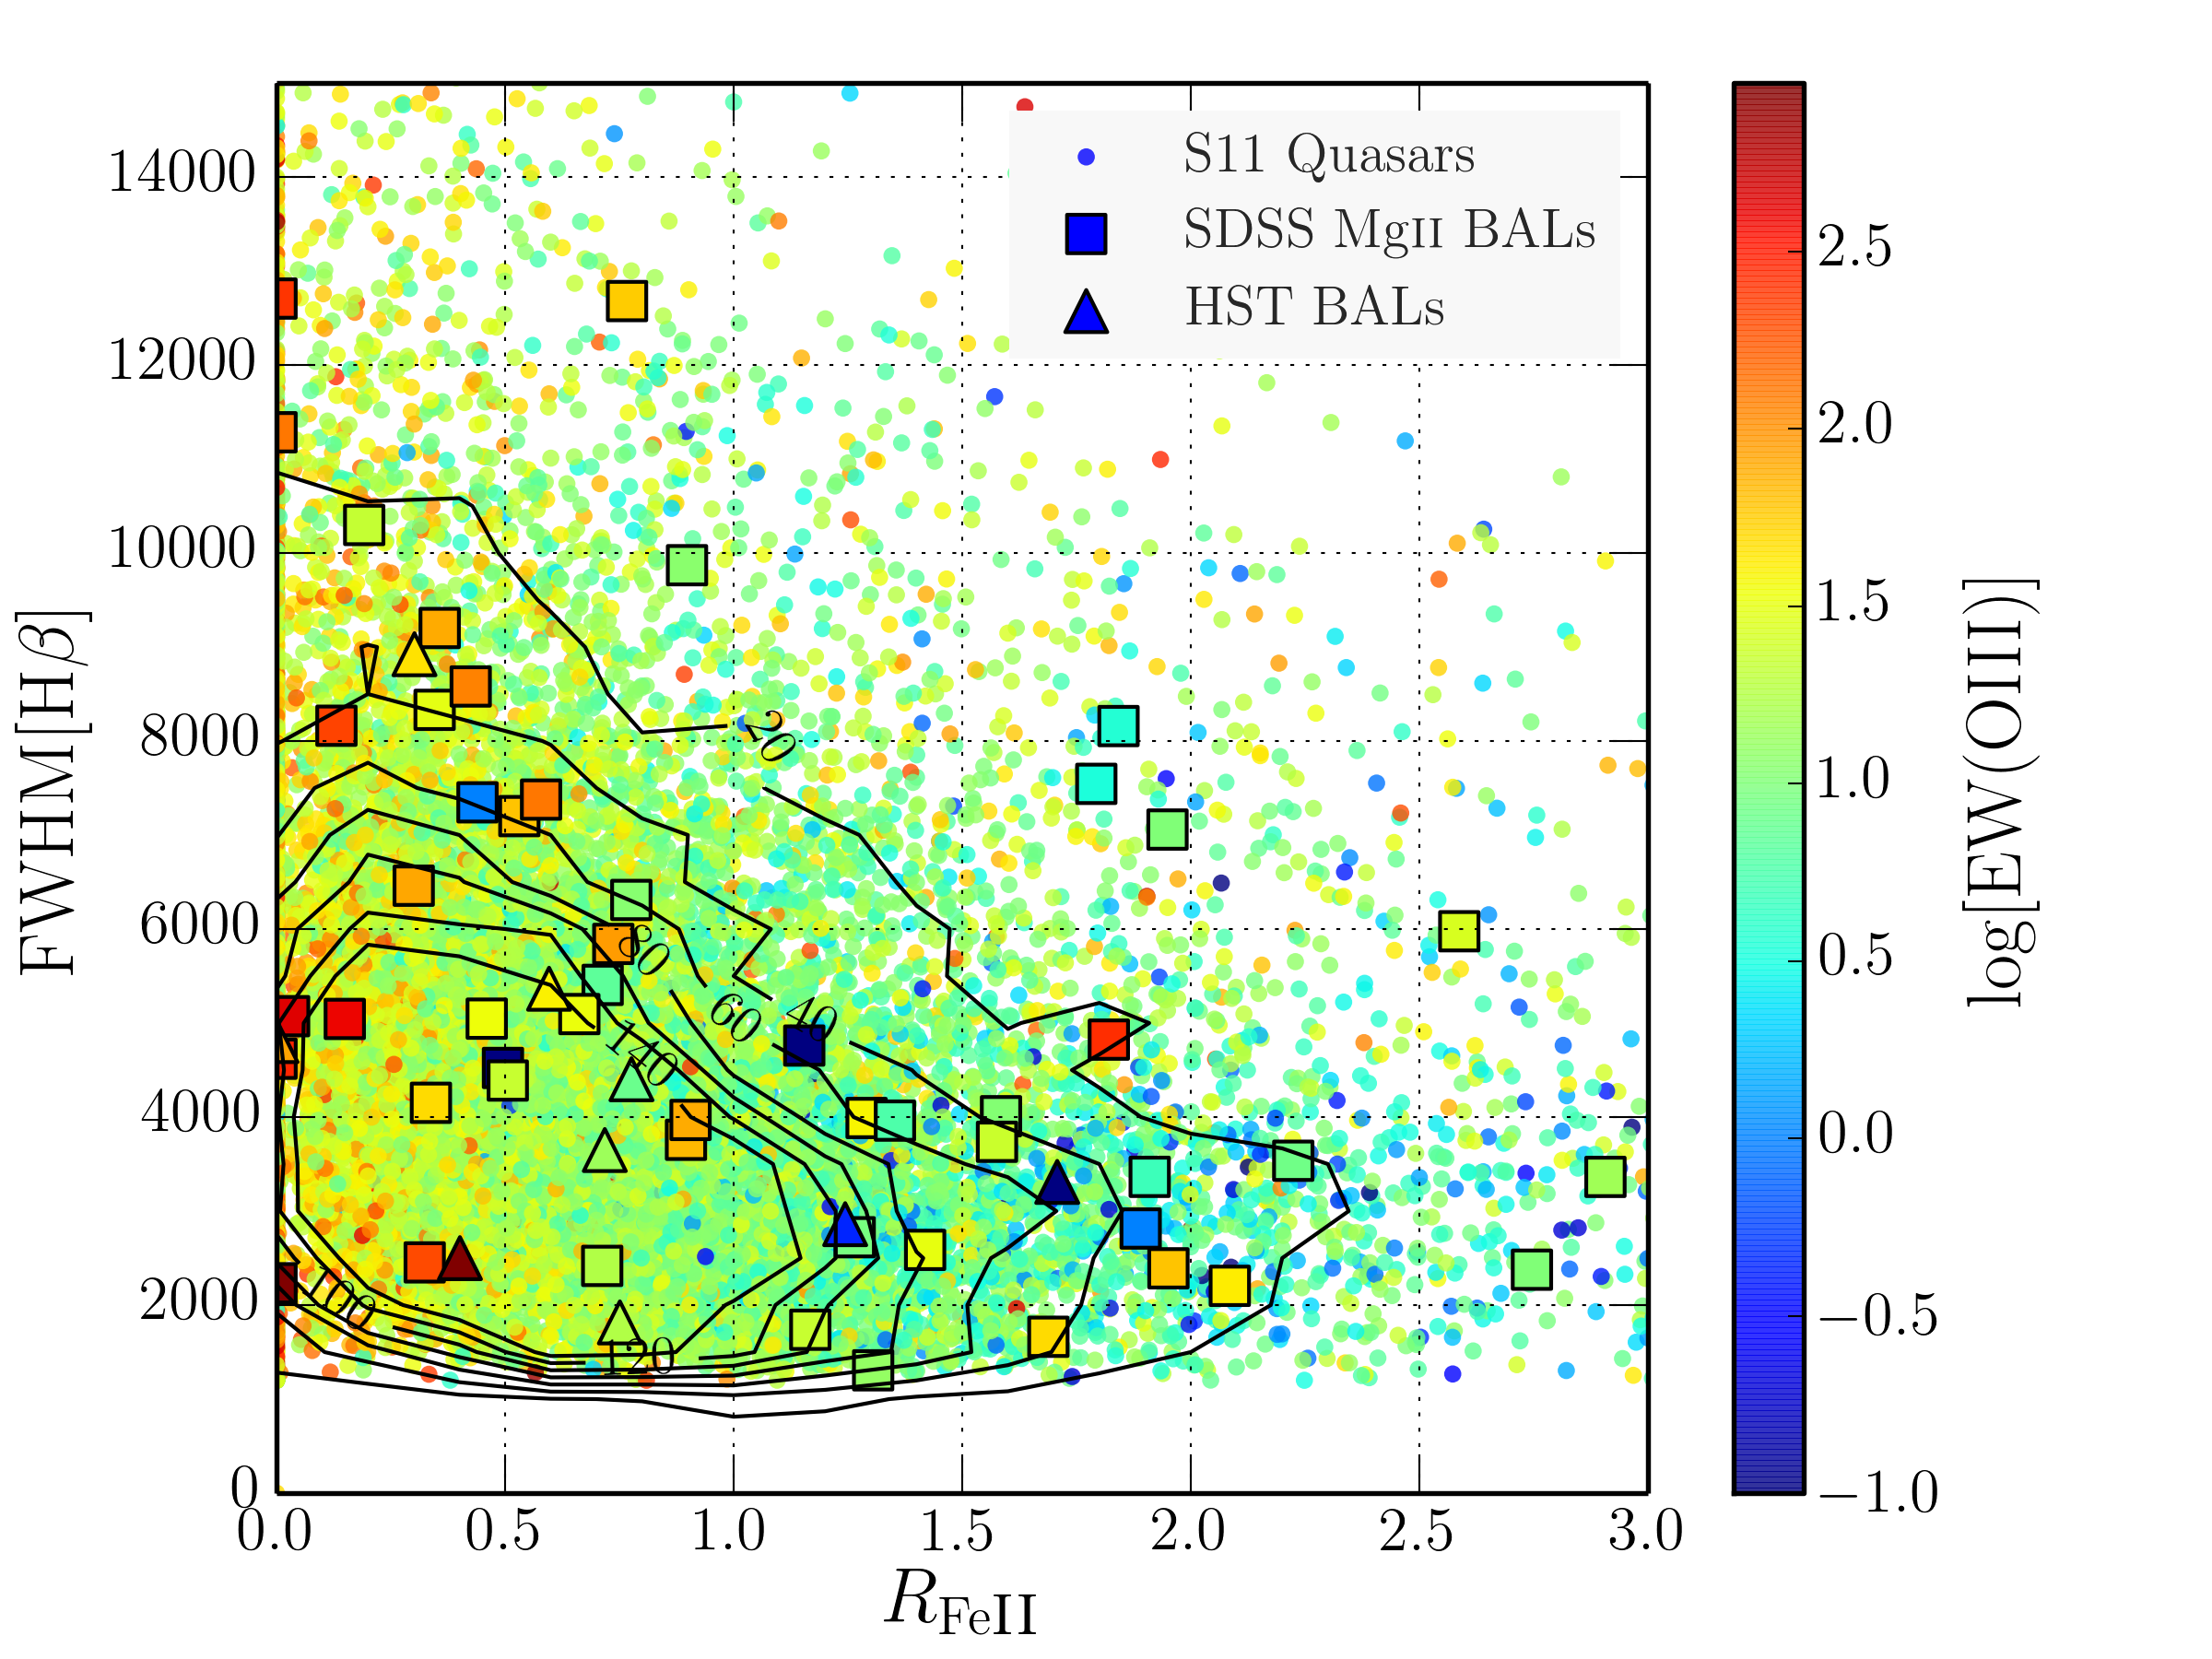
\includegraphics[width=1.0\textwidth]{figures/ewpaper/ev1.png}
\caption
[Eigenvector 1 for BAL and non-BAL quasars.]
{
Eigenvector 1 for BAL and non-BAL quasars. 
FWHM of the \hb\ line plotted against the relative
iron strength, $R_{{\rm Fe \textsc{ii}}}$. The colour coding
corresponds to the EW of OIII. The dots mark all quasars from
sample A, while the squares mark those with \mgii\ BALs.
The triangles show the HST BAL quasars from sample B.
}
\label{fig:bal_ev1}
\end{figure}

\begin{figure}
\centering
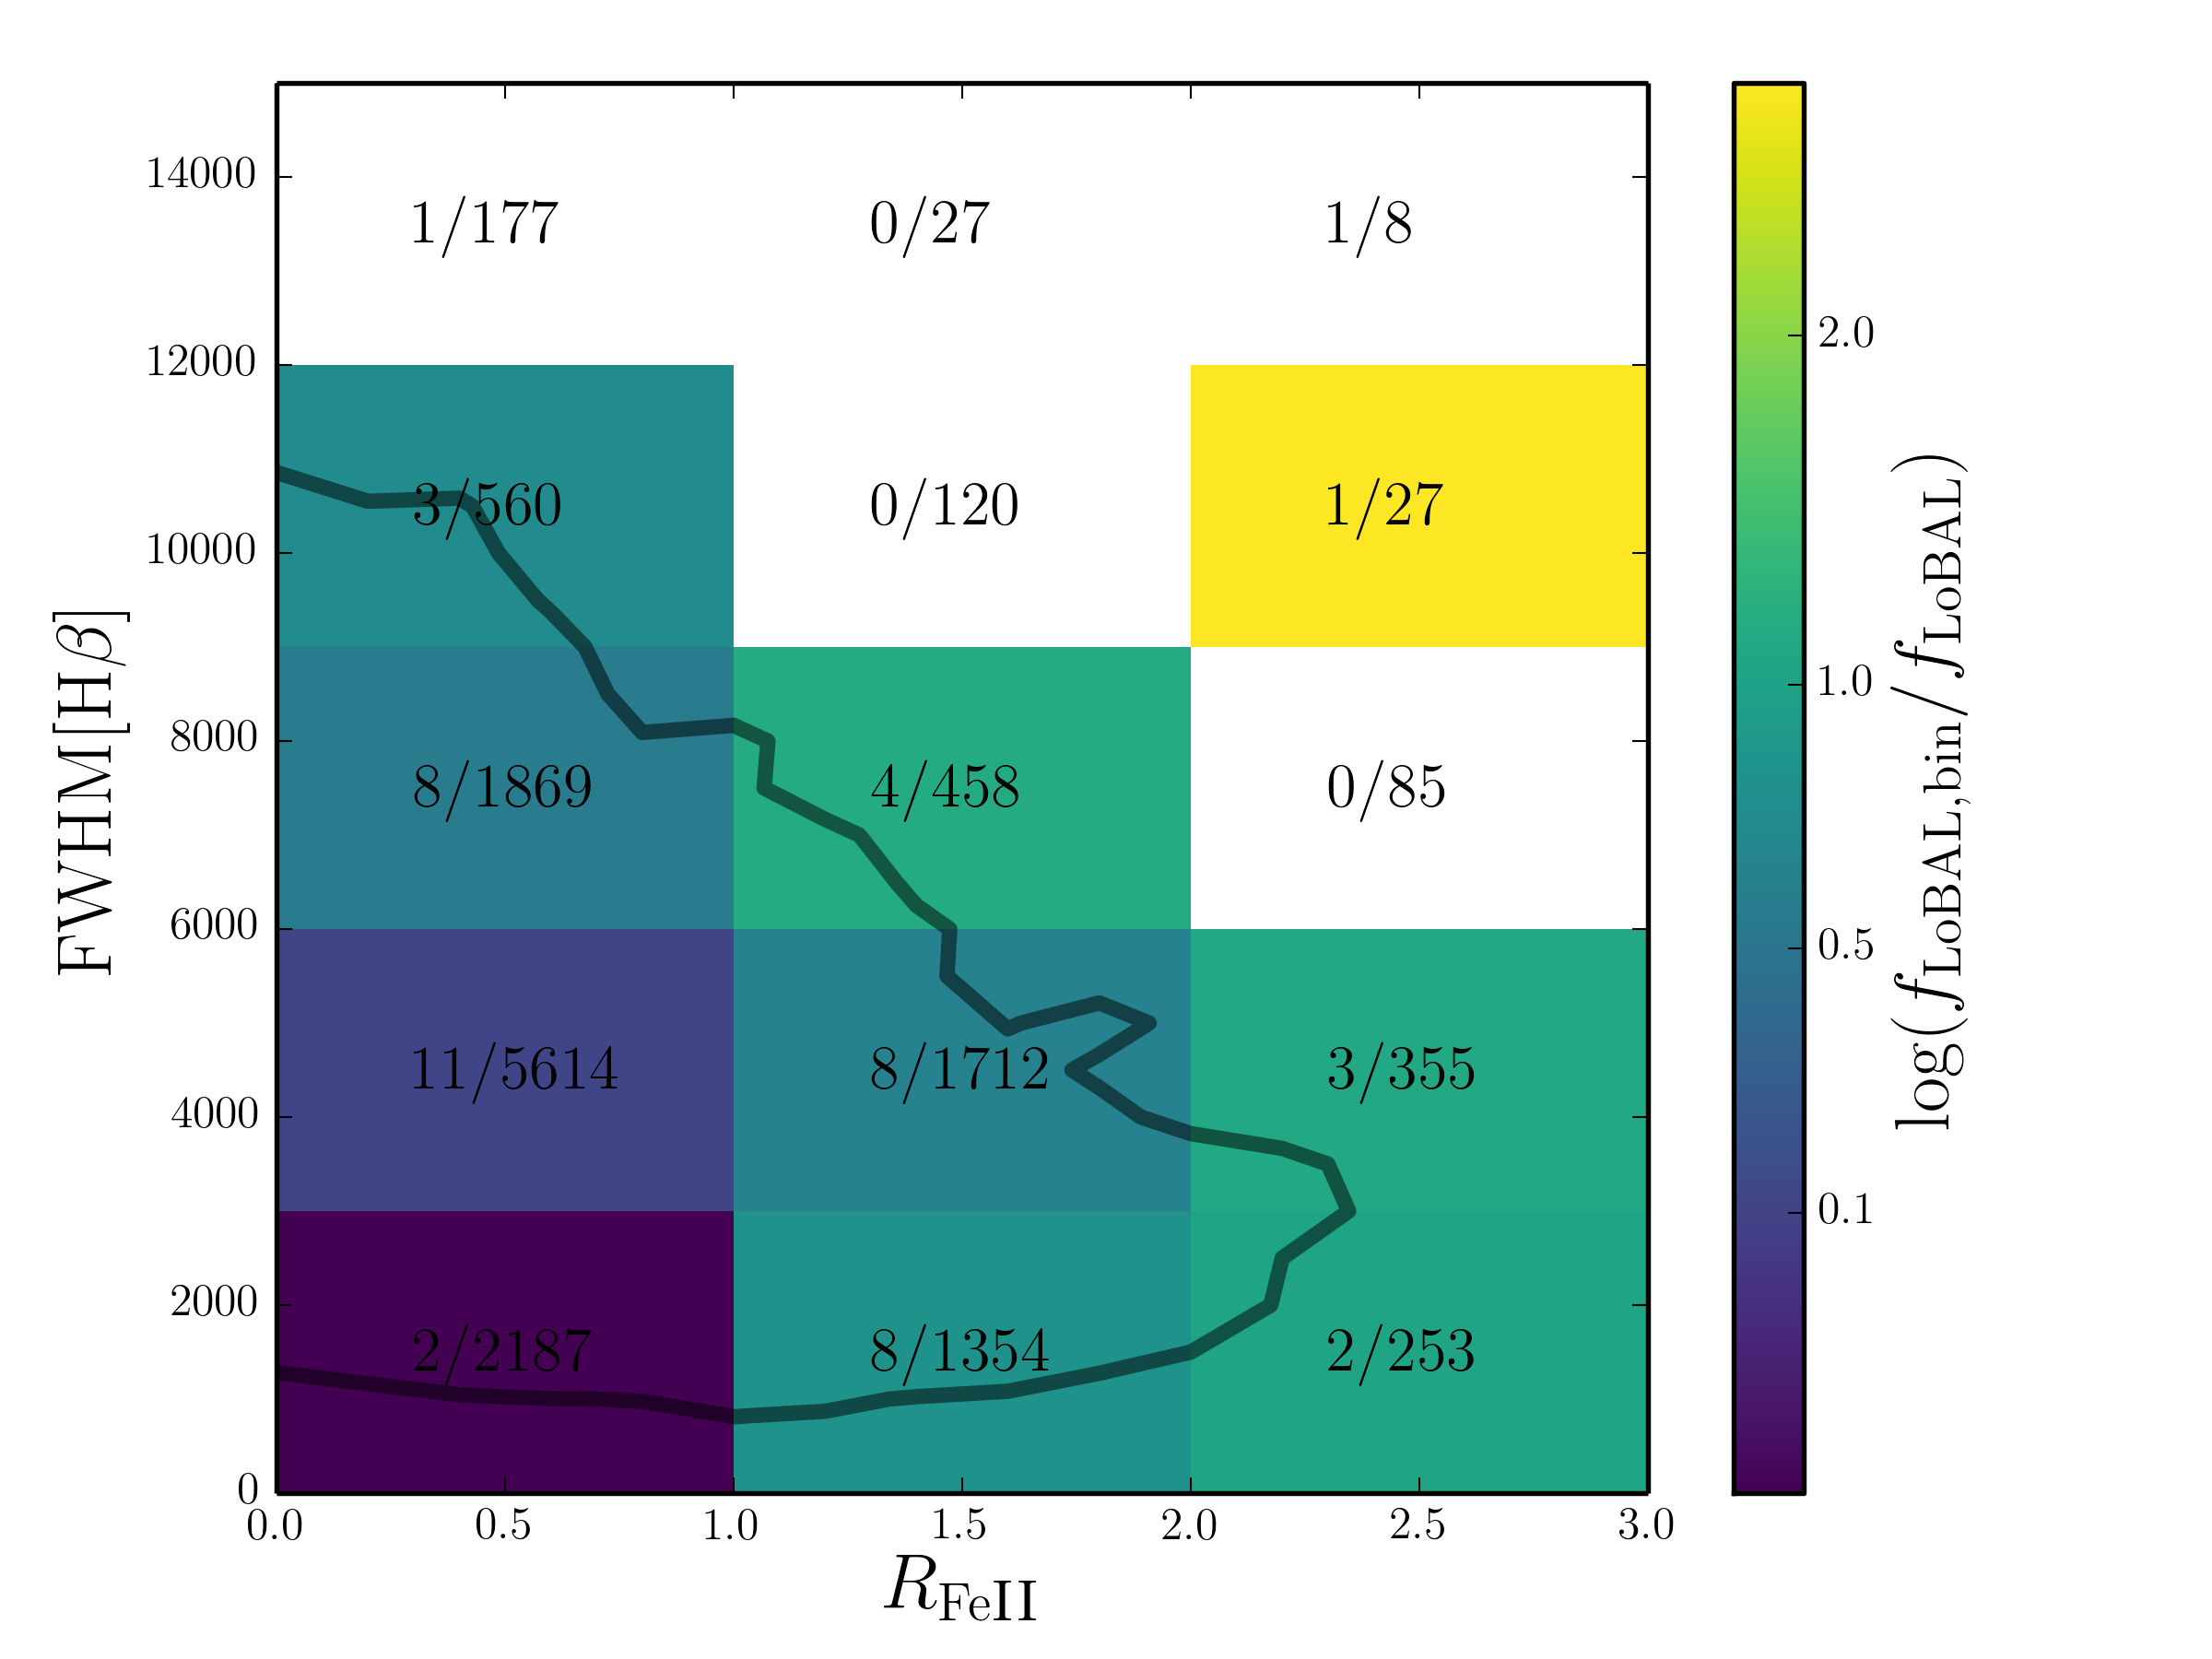
\includegraphics[width=1.0\textwidth]{figures/ewpaper/ev1_bins.png}
\caption
[LoBAL fraction compared to mean LoBAL fraction in Eigenvector 1 space.]
{
LoBAL fraction compared to mean LoBAL fraction in Eigenvector 1 space.
The contour shows the outermost contour from Fig.~\ref{fig:bal_ev1} for
reference.
}
\label{fig:bal_ev1_bins}
\end{figure}

% \begin{figure}
% \centering
% 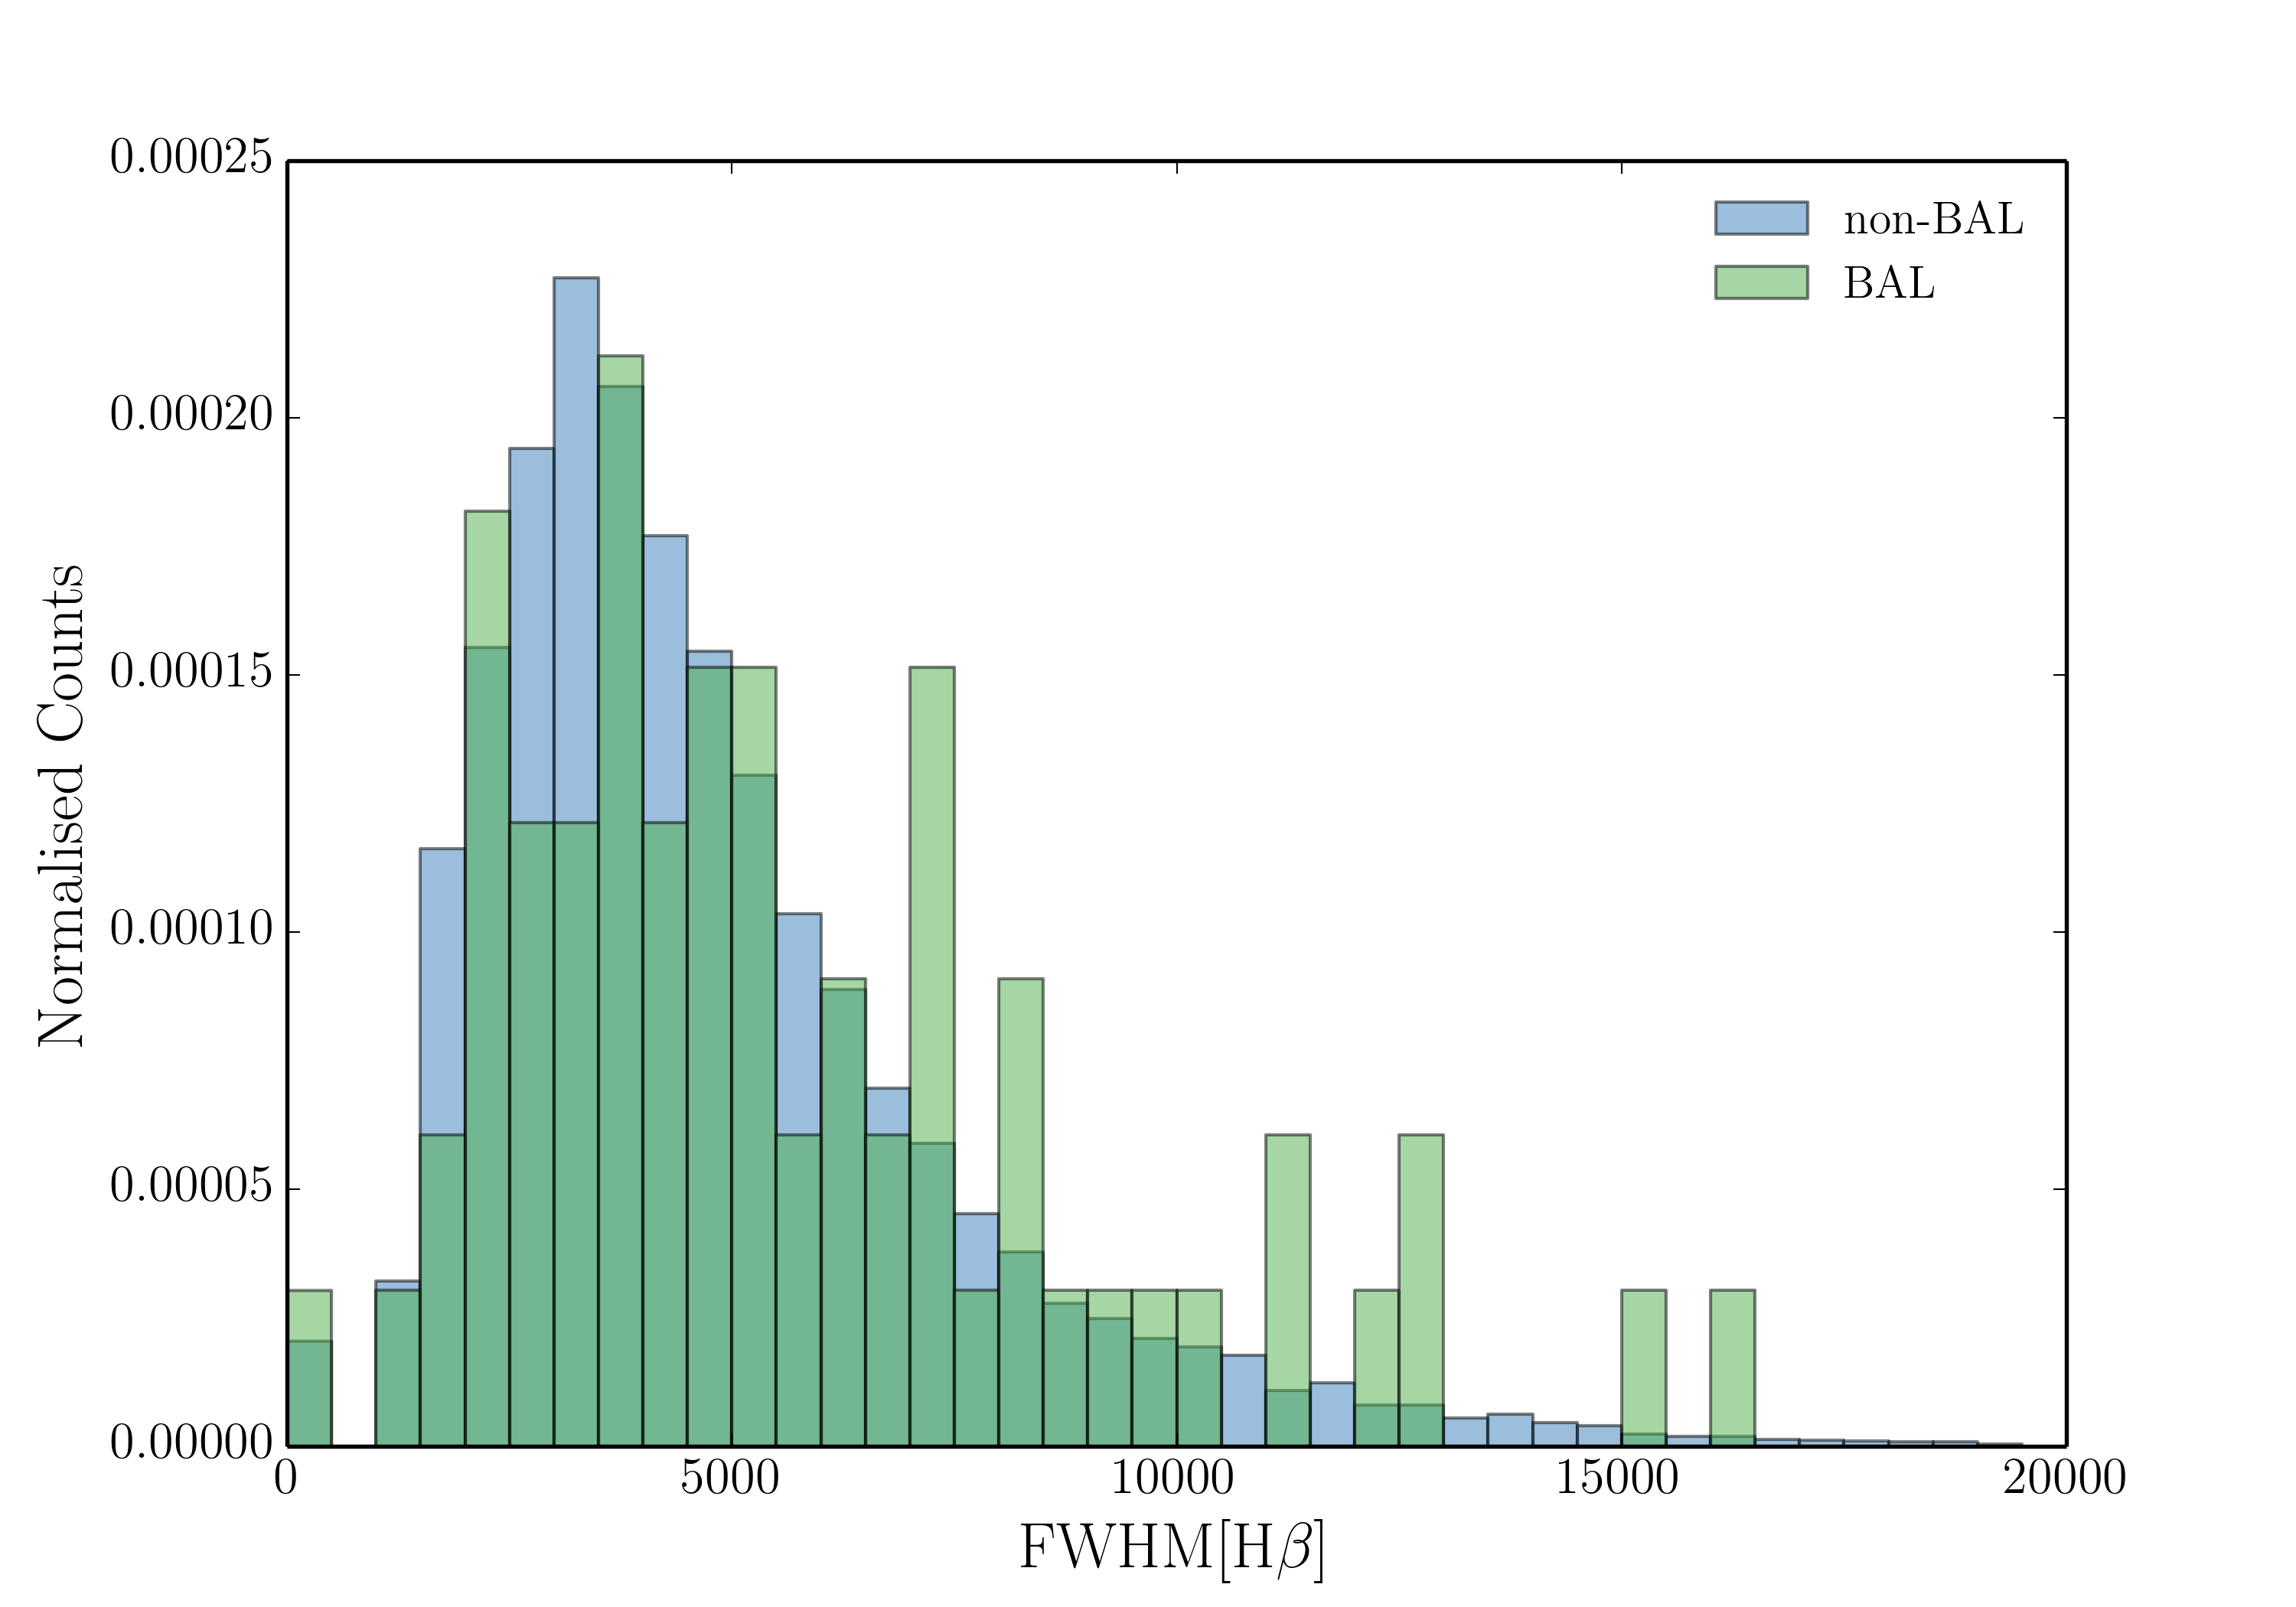
\includegraphics[width=1.0\textwidth]{figures/ewpaper/fwhm_hist.png}
% \caption
% [Distribution of \fwh\ in BAL and non-BAL quasars.]
% {
% Distribution of \fwh\ in BAL and non-BAL quasars.
% }
% \label{fig:fwhm_hb}
% \end{figure}

\subsection{Radio Observations}

Fig.~? shows the equivalent width distributions in radio-loud quasars, 
split into core or lobe dominated. This designation is commonly used
as an orientation indicator \citep{orr1982,wills1995}. 
Although th

In this case, we can see that 
A full investigation of this is beyond the scope 

% {\color{blue}
% Alternative geometries and polarisation. Are there any problems with
% a more moderate viewing angle for BALs? Do we want to show a cartoon?
% Discuss modelling work. Also discuss compton-thick fraction at high mass end.
% What about PHYSICS. Can we derive lower limits on outflow angles from
% e.g. conservation of angular momentum??
% }


\subsection{Polarisation}

Polarisation measurements of BAL quasars tend to show two properties.
The first is a polarisation angle of $\gtrsim60^\circ$ with respect
to the radio jet axis in RL source \citep{brotherton2006}. The second
is a polarisation percentage of around $2.4$ times greater, 
on average, than the 
non-BAL population. The polarisation percentages of a sample 
of BAL quasars from REF
are compared to the Type I and Type II AGN populations from REF in 
Fig.~\ref{fig:bal_polarisation}.

The polarisation properties of BAL quasars offer some of
the best insights into the geometries of BAL outflows, some of which
appear to be in contrast with the conclusions drawn from emission
line and radio properties.

\begin{figure}
\centering
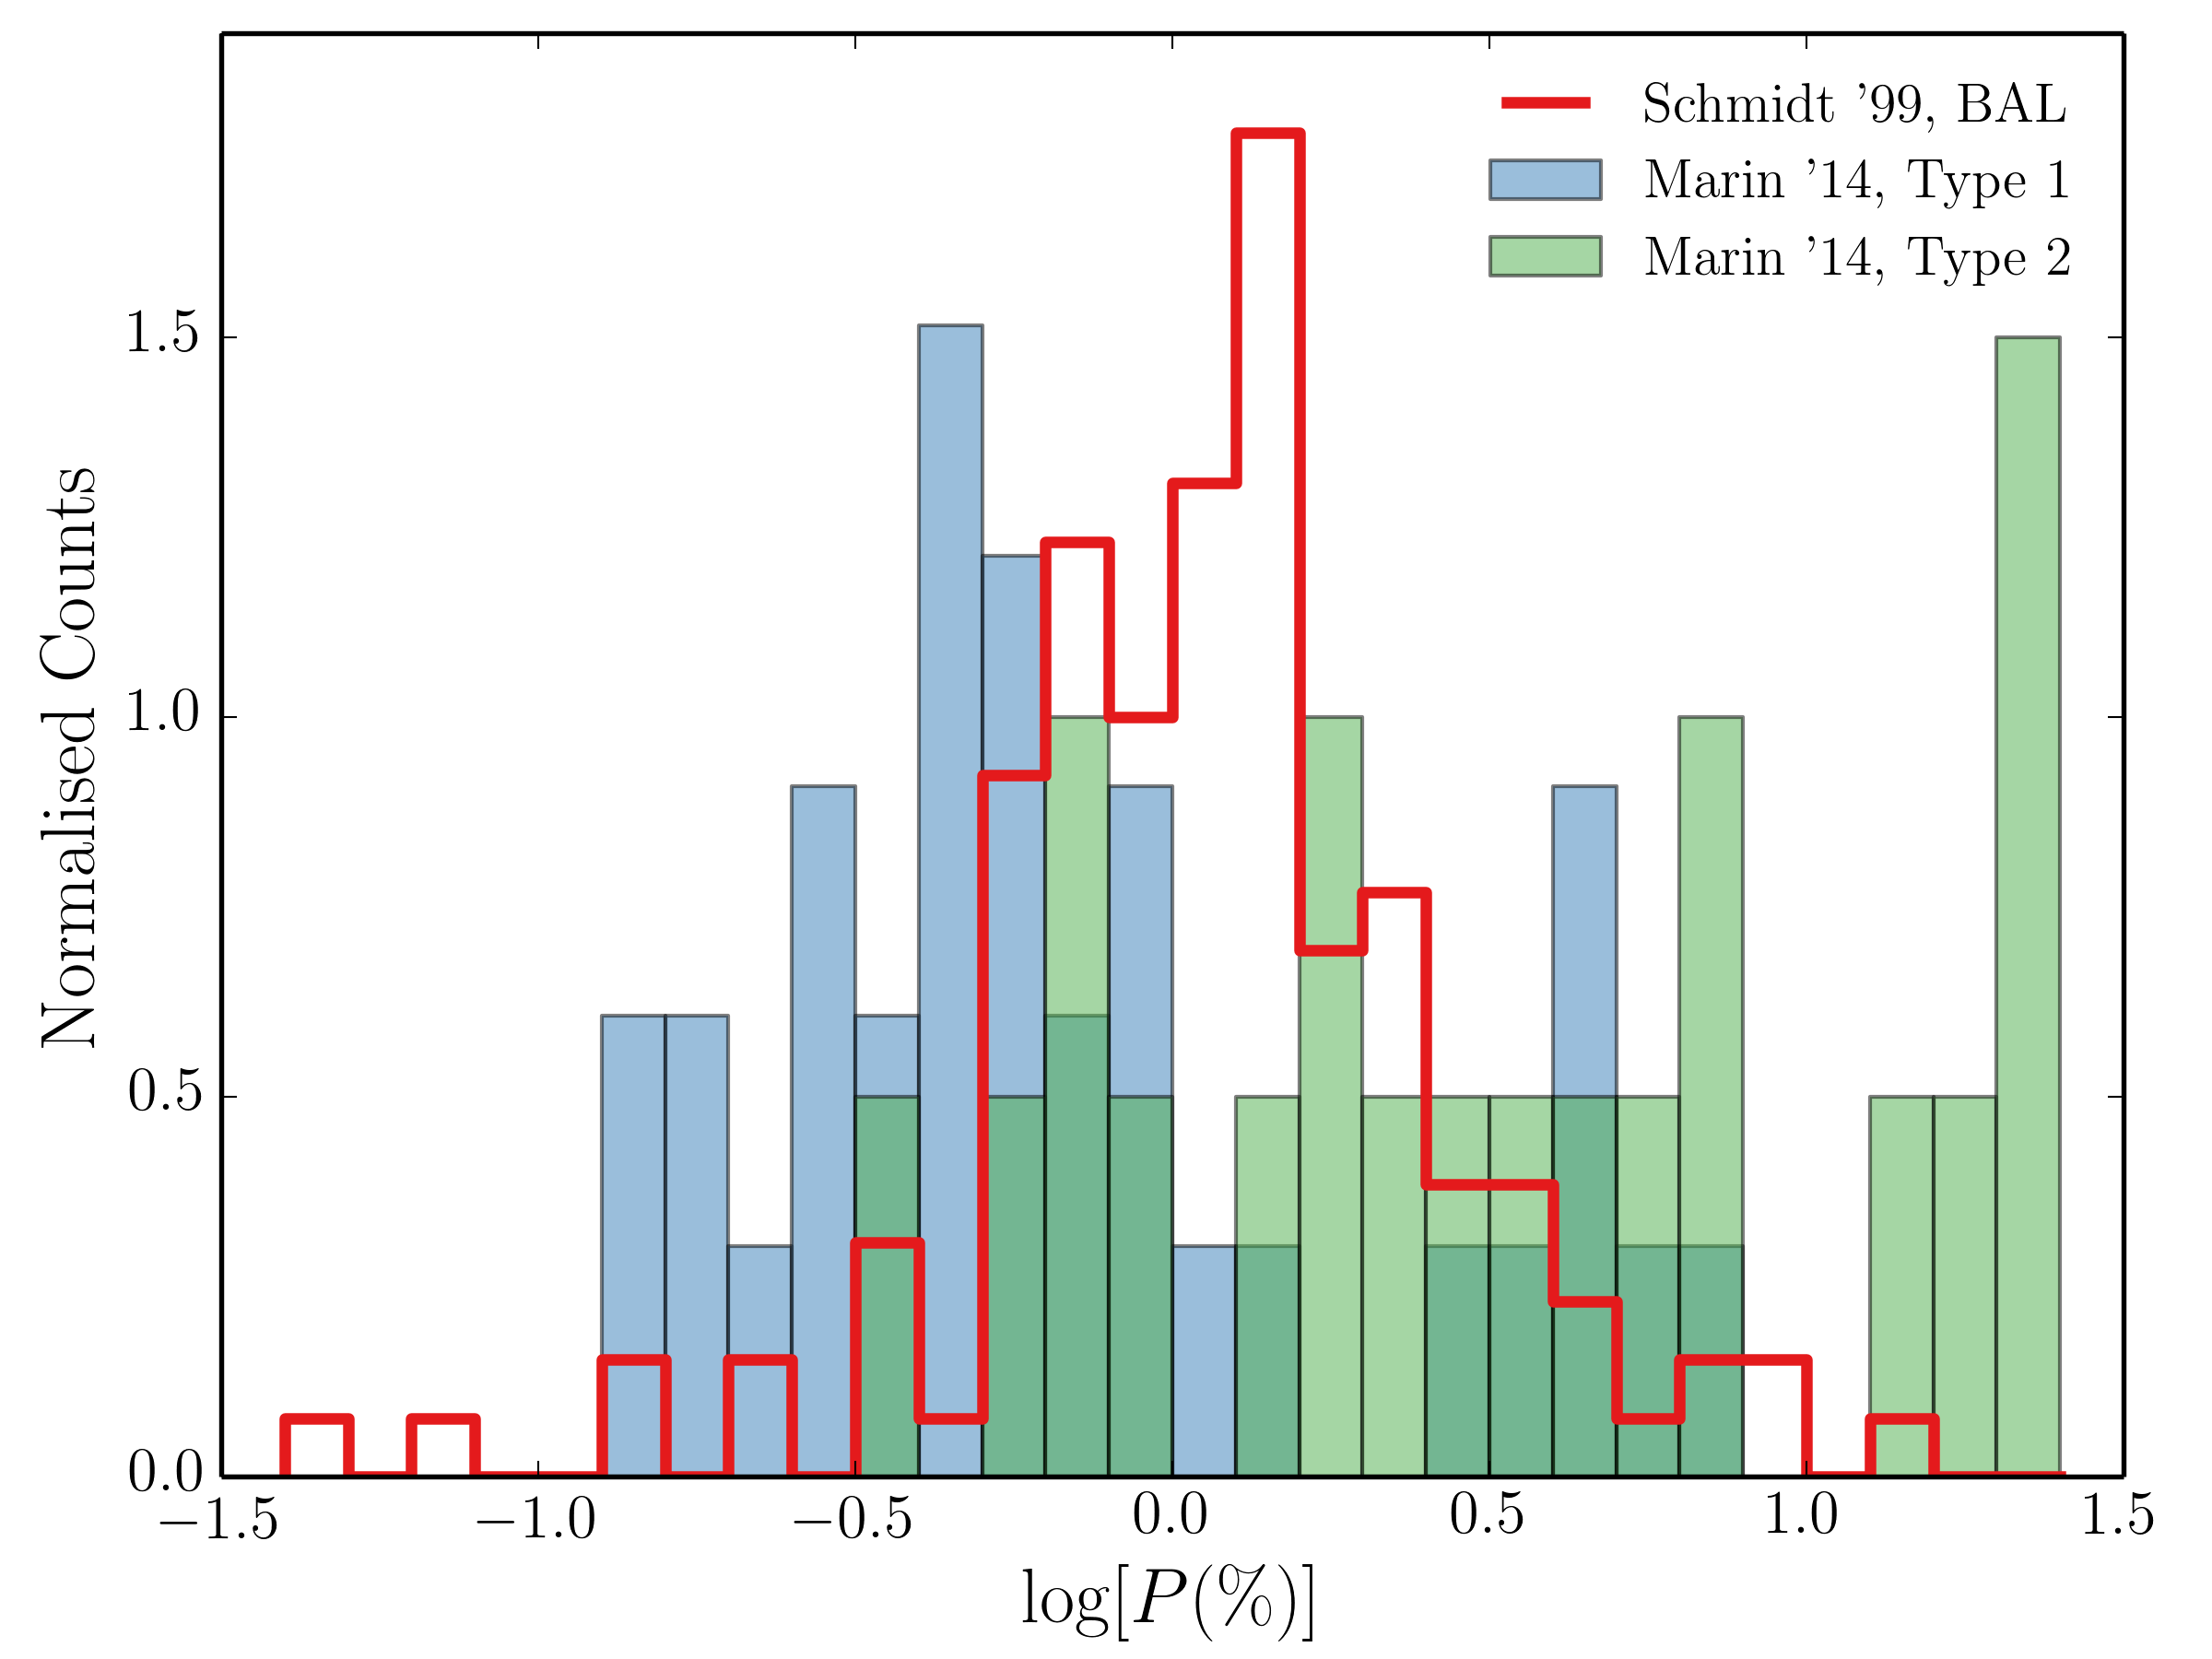
\includegraphics[width=1.0\textwidth]{figures/ewpaper/hist_p.png}
\caption
{
{\sl Top:} 
Polarisation percentages as a function of measured inclination from
Marin et al. (2015) for Type I and Type II AGN.
{\sl Bottom:} Histograms of polarisation percentages 
for BAL quasars from Schmidt et al. (1999) together with the 
Marin et al. (2015) AGN sample. 
}
\label{fig:bal_polarisation}
\end{figure}


\subsection{Theoretical Considerations}

Discuss Proga models: They tend to rise fairly equatorially (see eg. PK04) Talk to Nick?


\section{Conclusions}
\label{sec:ew_conclusions}
I have explored the emission line properties of BAL and non-BAL quasars 
and found that they are inconsistent with a unification picture in which 
BAL outflows rise equatorially from a foreshortened or limb darkened accretion
disc. Based on these findings, it is possible to 
construct a few possible scenarios that are not ruled out by the above results.
these conclusions have the caveat that I have assumed that conclusions drawn about
LoBAL quasars can be extended to BAL quasars in general.
\begin{itemize}
	\item {\sl Scenario 1:} The quasar continuum is roughly isotropic, which is not 
	expected from a geometrically thin, optically thick accretion disc.
    I have demonstrated that general relativistic effects cannot account for this discrepancy in the 
    UV. Reprocessing by surrounding dense plasma with a large covering factor or limb brightening 
    in the disc may provide possible explanations which this analysis cannot yet confirm or refute.
    \smallskip
	\item {\sl Scenario 2:} Quasar discs are strongly anisotropic, as expected from a 
	geometrically thin, optically thick accretion disc. In this case, BAL outflows cannot 
	only emerge at extreme inclinations and should instead be seen at very similar angles
	to non-BAL quasars. Polarisation measurements need to be reconciled with this hypothesis.
	I recommend that future RT modelling efforts explore different outflow 
	geometries and that detailed polarisation modelling is undertaken to constrain the 
	outflow opening angles.
	\smallskip
	% \item {\sl Scenario 3:} BAL outflows are more collimated than expected from early
	% polarisation measurements. This easily explains the emission line properties of BAL 
	% and non-BAL quasars. However, equatorial geometries have been most successful when modelling
	% BAL quasars, and there are clear differences in the polarisation properties of BAL and
	% non-BAL quasars. We recommend that future RT modelling efforts explore different outflow 
	% geometries and that detailed polarisation modelling is undertaken to constrain the 
	% outflow opening angles.
	% \smallskip
	\item  {\sl Scenario 3:} The geometric unification model does not explain the incidence of 
	BALs in quasars, or requires an additional component which is {\em time-dependent}, 
	such as an evolutionary or accretion state origin for BAL outflows. In this scenario, 
	BAL quasars would be seen from very similar angles to non-BAL quasars. However, the 
	evidence for this is limited and there is no good model for why outflows would exist 
	only for $\sim 20\%$ of a quasar's lifetime. Even if this is the case, then the covering 
	factor of the outflow still needs to be constrained in order to estimate the BAL duty cycle.
\end{itemize}
Regardless of the conclusions about BAL quasars and their outflow geometries,
this analysis allows conclusions to be drawn about the {\em overall} 
quasar population. In scenario 1, the \ewo\ distribution of quasars cannot
be driven by inclination as suggested by \citep{risaliti2011}. 
It is also clear from the work presented here that $\log R$, \ewo\ and FWHM \hb\ 
are {\em cannot all} be reliable orientation indicators. 
Furthermore, if a geometric unification does explain BAL quasars, then 
absorption effects cannot be responsible for the observed \ewo\ distribution.
The above conclusions each pose a different challenge to the current
understanding of, respectively, accretion physics, polarisation measurements 
and geometric unification models. This work therefore adds to the
growing evidence that our simplest models are not sufficient to
describe the overal quasars and that alternatives should be sought.


